\documentclass[oneside,chapterprefix=on,12pt,parskip=full,bibliography=totoc]{scrbook}  %chapter prefix is to make chapter appear in titles. parskip is to have lines between paragraphs with no indentation, bibliography=totoc lists bibliography in contents.
\usepackage[top=2.5cm, bottom=3.2cm, left=2cm, right=2.0cm]{geometry} 
\usepackage[utf8]{inputenc}
\usepackage{amsmath}
\usepackage{amsfonts}
\usepackage{amssymb}
\usepackage{graphicx}
%\usepackage[retainorgcmds]{IEEEtrantools}
\numberwithin{equation}{section}
\usepackage{cite}
\usepackage[onehalfspacing]{setspace}
\usepackage[titletoc]{appendix}
\usepackage{braket}


\setlength{\headheight}{1.1\baselineskip} %To do with space for header at chapter titles.



\renewcommand{\autodot}{}% Remove all end-of-counter dots


%\usepackage{caption} 
%\captionsetup[table]{skip=8pt}

% set up page. "headmark" is to have chapter titles at top of page. "pagemark" is page numbers i/c/o are right,centre,left
% square brackets for title pages. curly brackets for normal pages
\usepackage{scrpage2}
\pagestyle{scrheadings}
\ihead[]{\headmark}
\chead{}
\ohead[]{}
\ifoot[]{}
\cfoot[\pagemark]{\pagemark}
\ofoot[]{}


\renewcommand{\bibname}{References} %By default this class calls it Biliography. Change it to References here.



\begin{document}

\begin{titlepage}
\centering
\vspace*{1in}
\begin{Large}\bfseries
TROVE Manual\par
\end{Large}
Version 1 \par
\vspace{1.5in}
\begin{large}\bfseries
Barry Mant\par
\end{large}
\vfill
\vspace{0.5in}
Department of Physics and Astronomy
\par
University College London
\par
\vspace{0.5in}
June 2018
\par
\end{titlepage}

%\maketitle

\frontmatter



\chapter{Abstract}
A guide to TROVE.


% A glossary and list of acronyms may go here
% or may go in the back matter.


\doublespacing        %Double spacing contents and lists as looks cramped otherwise
\tableofcontents
%\listoffigures
%\listoftables

\mainmatter
\onehalfspacing      %One halfspacing from here again


\chapter{Introduction}
\label{sec:intro}

\section{What is TROVE?}
\label{sec:whatsTrove}
TROVE (Theoretical ROtational Vibrational Energies) is a suite of programs primarily designed for the 
calculation of molecular infrared line lists\cite{TROVE}.
It was (and is) developed by Sergey Yurchenko with contributions from others over the years. 
It has been used to study a range of molecules and features continue to be added. 

The main capabilities of TROVE are as follows: The calculation of rotational-vibrational energy levels of polyatomic molecules; 
Refinement of \textit{ab initio} potential energy surfaces (PES) using experimental data;
The calculation of infrared transition intensities and absorption cross sections. 

The philosophy of TROVE is to enable the study of molecules of arbitrary structure. 
This is possible since TROVE uses a numerically generated Hamiltonian unlike other programs which are hard coded with 
specific analytical Hamiltonians. 
So far TROVE has been used for diatomics,\cite{TROVE} triatomics,\cite{TROVE} tetratomics,
\cite{jt466,jt500,jt554,jt553,jt556,jt597,jt592}
pentatomics\cite{jt564,jt612,jt701} and hexatomic molecules\cite{jt729}
and there are plans to implement even larger molecules. 
The structure of TROVE also allows very straightforward studies of new molecules of the same structure and symmetry to
molecules which have previously been implemented. For example, since phosphine, PH$_3$ is implemented, it is simple to then
carry out calculations on arsine, AsH$_3$, provided a PES and dipole moment surface (DMS) is available. 

TROVE calculates rotational-vibrational energy levels using the variational method.\cite{11Atkins.book}
In very simple terms this method requires a suitable choice of functions called a basis set, 
the calculation of a Hamiltonian matrix using the basis set and the diagonalisation of the Hamiltonian. 
The eigenvalues are the energy levels for the system while the eigenfunctions are the states/wavefunctions of the system. 
TROVE carries out this procedure in a very sophisticated manner by building up basis sets from calculations on smaller 
parts of the system and makes use of symmetry to simplify the calculation of matrix elements and reduce the size of 
matrices to be diagonalised. Despite the complexity of the implementation in TROVE, the basic procedure should be 
kept in mind.  

\section{What is this manual for?}
This aim of this manual is to describe the theory behind TROVE and especially how to operate TROVE in more detail than
would be possible in a journal publication. Since the original paper, many new features have been added to TROVE which have
been described as they were applied. In this manual these new features will be described in one place in more detail.

TROVE is very much a `living' program with new capabilities being added all the time. This may mean that some parts of 
this manual are not be up to date or even superfluous for the reader. Nevertheless, it is anticipated that the core
parts of TROVE will not change significantly and that this document will still be of use, especially to new
TROVE users. The last chapter describes new features of TROVE and will be kept up to date with new developments. 


The `Quick start' chapter following this one is aimed at new users, especially new PhD students and postdocs, to get 
 started doing calculations with TROVE assuming some set up has already been done for the molecule of interest. 
Later chapters describe the underlying theory behind TROVE, a detailed description of outputs, the refinement procedure,
the calculation of line lists, a list of molecules already implemented in TROVE and summary of work on them, 
how to set up TROVE for a new molecule and finally, new features in TROVE. 










\chapter{Quickstart}
\label{chap:Quickstart}
The aim of this chapter is to get a new TROVE user, especially PhD students and postdocs, up 
and running with the program to enable them to start carrying out calculations. 
It is assumed that for the molecule of interest, the molecular symmetry and geometric transforms have already been defined 
and that a PES and DMS has been implemented. 
If this is not the case then see later chapters for how this is carried out. 

TROVE inputs will be treated in a general manner with occasional examples given for 
the phosphorus trifluoride molecule, PF$_3$. This molecule has the same trigonal pyramidal shape as ammonia but 
without the complication of tunnelling inversion. This is a `rigid molecule', for molecules with a non-rigid degree of 
freedom, see later chapters. A `typical' way TROVE is used to go from vibrational calculations 
to full line lists is also given. 


\section{Input File Keywords and Check Point Files}
The TROVE input file is structured in blocks with keywords within each block controlling options and parameters
of the calculation. 
These blocks will be described individually along with a description of the checkpoint file structure. 
A full input file for PF$_3$ is given at the end of the chapter.

\subsection{Memory Allocation}
The total working memory which TROVE can use in a calculation is specified by 
\begin{verbatim}
mem 20GB
\end{verbatim}
where in this case TROVE could use 20 GB of RAM. If no \verb|mem| command is given TROVE will 
assume the whole CPU memory is available which can cause problems if running on a shared memory computer. When running TROVE
on such machines it is recommended that the memory is set to the combined memory of the number of cores being used.  

\subsection{Kinetic and Potential Energy Expansion Order}
As described in more detail in later chapters, TROVE numerically generates the Hamiltonian using internal coordinates. 
The kinetic energy operator and potential energy of a molecule are expanded up to a given order 
The order of this expansion is specified by the keywords
\begin{verbatim}
KinOrder i
PotOrder j
\end{verbatim}
where \verb|i| and \verb|j| are integers. The larger these integers are, the more accurate an expansion 
of the Hamiltonian is produced. 
For fast, test calculations, setting \verb|i| and \verb|j| to 2 and 4 respectively should be sufficient. 
For accurate results \verb|i| and \verb|j| should be set to 6 and 8 or 8 and 10 respectively.\cite{TROVE} 

A possible problem which can arise here is the order of expansion of the potential energy. 
It may be that calculations are fine for low orders but on increasing the expansion order TROVE reports problems 
with the primitive one-dimensional Numerov basis functions (see below). 
This can occur if the potential expansion `turns over' leading to a poor representation of the potential as shown
in Figure \ref{fig:pot_exp}.
Remedies for this problem are increasing \verb|j| to a sufficient value or reducing the range the Numerov basis is 
generated over. 

\begin{figure}[h!]
	\centering
	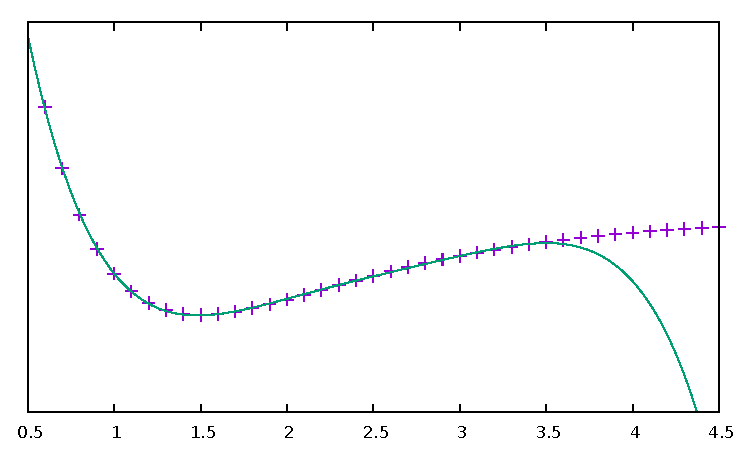
\includegraphics[scale=0.8]{pot_expand} 
	\caption{Illustration of how expansion (line) of actual potential (crosses) can fail.}
	\label{fig:pot_exp}
\end{figure}

\subsection{Number of Atoms and Modes}
The number of atoms and vibrational modes is defined by the keywords
\begin{verbatim}
Natoms n
Nmodes i
\end{verbatim}
where \verb|i| is normally 3\verb|n|$-$6 for non linear molecules and 3\verb|n|$-$5 for linear molecules.

\subsection{Primitive Block}
The polyad number and maximum energy for the primitive basis functions are set in the primitive block:
\begin{verbatim}
PRIMITIVES
Npolyads p
enercut  x
END
\end{verbatim}
As discussed in more detail in later chapters, TROVE uses products of primitive one-dimensional functions as basis functions. 
The polyad number, $P$, is a way to restrict the size of the basis set.\cite{TROVE} 
The sum of the primitive function's vibrational quantum number, $v_i$, is then restricted to be below \verb|n|, that is:
\begin{equation}
\label{eq.polyad}
P = \sum_i a_i v_i \le n.
\end{equation}
where $a_i$ is an integer used to control the basis further.
For fast, test calculations a low value of \verb|n| should be used, for example 4. 
Increasing n gives a larger basis set which will give more accurate results (and extend the energy range) 
at the expense of time and memory.
Note that because of how the polyad number is defined, even increasing \verb|n| by 1 can lead to a much larger basis.

Another way of limiting the size of the primitive basis functions is by energy. 
The \verb|enercut| keyword specifies the maximum energy a primitive basis function can have if it is to be included. 
As discussed below, the basis set is further restricted by energy in the Contraction block and so usually \verb|x|
 is set to a large value. For example 40,000 (in units of wavenumbers, cm$^{-1}$). 

\subsection{Contraction Block}
As will be discussed in later chapters, TROVE builds contracted basis functions from the primitive basis functions. 
In the Contraction block the parameters for making this contraction are chosen. A Contraction block example is 
\begin{verbatim}
CONTRACTION
  Npolyads        n
  enercut         x
  coeff_thresh    1.0d-30
  degeneracy      1d-02
  sample_points   40
  sample_attempts 500
  symm_toler      1.0d-3
END
\end{verbatim}
\verb|Npolyads| is the same as for the Primitive block and defined in equation \ref{eq.polyad} 
and sets the maximum polyad number for the contraction. 
Similar to the primitive block, \verb|enercut| sets the maximum energy a contraction can have. The value of \verb|enercut| chosen depends on the application. 
Because the maximum energy of the contracted basis functions are set, it makes sense to set the value of \verb|enercut| in the Primitive block large.

Also given in the Contraction block are parameters relating to how TROVE works out the symmetry
of contracted basis functions (\verb|coeff_thresh, degeneracy...|). This will be described in later chapters and has been discussed in a recent publication \cite{17YuYaOv.methods}.


\subsection{Symmetry}
The symmetry of the molecule is specified by the \verb|SYMGROUP| keyword. 
The symmetry of a given molecule is set in the .mol file which, as ever, will be discussed in later chapters. 
For PF$_3$ the \verb|SYMGROUP| is set using
\begin{verbatim}
SYMGROUP C3v(M)
\end{verbatim}

\subsection{Diagonalizer Block}
The Diagonalizer block determines the way in which the Hamiltonian matrices are diagonalized. 
The method of carrying out the diagonalization is specified by a keyword related to the LAPACK/BLAS program which are used.
These are standard programs used for carrying out matrix manipulations used in many areas of science, engineering, mathematics,
etc. 
\verb|SYEV| is the default value which computes all eigenvalues and eigenvectors. \verb|SYEVR| allows an uppervalue on the computed eigenvalues to be specified.
There is another keyword, \verb|enermax|, which limits the energies of eigenfunctions which are saved. For example
\begin{verbatim}
DIAGONALIZER
 SYEV
 enermax 16000.0
end
\end{verbatim}
If a pure vibrational calculation (J = 0) is being carried out, 
the energies of excited states are automatically given relative to the zero point energy (ZPE) of the ground vibrational state. 
For J $>$ 0 calculations, the keyword \verb|ZPE| followed by the vibrational zero point energy should be specified 
so that rotational-vibrational energies are also given relative to the ground state.

For large calculations, it is more efficient to diagonalize each symmetry's Hamiltonian matrix separately. The symmetry of 
interest is specified using the keyword \verb|gamma n| where \verb|n|=1,2.. is the symmetry of interest.

\subsection{Print Out Level}

The amount of output printed is specified by the \verb|verbose| keyword. A value of 4 is sufficient for most purposes.
\begin{verbatim}
verbose 4
\end{verbatim}
Increasing this value will produce more output, this is useful for debugging, etc.

\subsection{Specifying the Molecule}
The molecule is defined in TROVE by the following
\begin{verbatim}
dstep            0.01
COORDS           linear
TRANSFORM        r-alpha
MOLTYPE          XY3
MOLECULE         PF3
REFER-CONF       RIGID
\end{verbatim}

\verb|dstep| has to do with how fine a grid TROVE carries out the coordinate transform on.

The \verb|COORDS| keyword specifies the type of internal coordinates. The standard option is \verb|linear| which indicates 
that the kinetic and potential energy should be expanded in linear coordinates \cite{TROVE}. 
Another option is \verb|local| which 
uses curvilinear coordinates \cite{15YaYuxx.method}. Currently curvilinear coordinates are not a part of `standard' TROVE. 

\verb|TRANSFORM| specifies how to transform the coordinates from Z-matrix to the coordinates used in TROVE.
This is specified in the .mol file for the molecule of interest.
For the PF$_3$ example here, the details of the transformation are given in the `r-alpha' subroutine.

As the symmetry transforms only need to specified for each type of molecule of the same symmetry, they can be reused. 
For example PCl$_3$ belongs to the same symmetry
group as PF$_3$. The \verb|MOLTYPE| keyword identifies the `type of molecule' and molecules of the same symmetry can 
then be straightforwardly used. This keyword specifies the subroutine to use to define rotational symmetries, etc.

\verb|MOLECULE| is an optional keyword which specifies the molecule's name.

Whether the molecule is `rigid' or `non-rigid' is specified with the \verb|REFER-CONF| keyword. For non-rigid molecules
a special degree of freedom which is large amplitude (or `floppy') can be specified. Examples include the inversion
motion in ammonia or the torsional motion in ethane. In this case HBJ theory (see Theory chapter) can be used.




\subsection{Z-Matrix Block}
The Z-matrix block specifies the molecule's geometry and masses of atoms. For example for PF$_3$ the Z-matrix is
\begin{verbatim}
ZMAT
    P   0  0  0  0   30.973761998
    F   1  0  0  0   18.998403162
    F   1  2  0  0   18.998403162
    F   1  2  3  0   18.998403162
end
\end{verbatim}
The Z-matrix used by TROVE is very similar to those used by electronic structure programs such as Molpro 
and Gaussian.\cite{06Jensen.book}
The first column is the atom's (element) symbol. The second column is the atom which the atom of that row is connected to. 
The third column is the bond angle between the atom of the row and a specified atom. The fourth column is the dihedral angle 
between the atom of that row and a specified atom. The fifth column has to do with the way a particular molecule type is
set up in TROVE and describes the type of dihedral angle. The sixth column is the atom's mass in atomic mass units. 
Note that isotope masses should be used, not averaged atomic weights. 


\subsection{Basis Block}
The Basis block specifies the type of basis functions used by TROVE and how the kinetic and potential energy is expanded
for each coordinate.
Specifically, the one-dimensional basis functions which will then be used to build up contracted and symmetrized functions. 
An example for PF$_3$ is 
\begin{verbatim}
BASIS
0,'JKtau', Jrot 0
1,'numerov','linear','morse',range 0,7, resc 2.0, points 2000, borders -0.4,2.0
1,'numerov','linear','morse',range 0,7, resc 2.0, points 2000, borders -0.4,2.0
1,'numerov','linear','morse',range 0,7, resc 2.0, points 2000, borders -0.4,2.0
2,'numerov','linear','linear' range 0,14, resc 1.0, points 2000, borders -1.3,1.3
2,'numerov','linear','linear',range 0,14, resc 1.0, points 2000, borders -1.3,1.3
2,'numerov','linear','linear',range 0,14, resc 1.0, points 2000, borders -1.3,1.3
END
\end{verbatim}
The first line in this block, \verb|0,'JKtau', Jrot 0| specifies the rotational functions. 
For $J>0$ calculations the value of \verb|Jrot| is changed to $J$ of interest.
PF$_3$ has $3N - 6 = 3(4) - 6 = 6$ internal degrees of freedom and thus 6 basis functions are required. 
Basis functions are grouped using an integer label.
For this example, '1s' are the P-F stretches and '2s' are the P-F bends. The grouping is used for producing symmetric 
combinations of basis functions and only coordinates symmetrically related should be grouped together. Details of this
procedure are discussed in the Theory chapter and in a recent paper \cite{17YuYaOv.methods}.

For a given basis function row the options are as follows. The first keyword specifies what the one-dimensional basis 
functions are. In this example they are numerically generated using the Numerov-Cooley method. 
Other options are `harmonic' and `morse' where these analytical basis functions shall be used.
The second keyword specifies how the kinetic energy operator is expanded.
The third keyword gives the expansion coordinates for the potential. Here 'Morse coordinates' of the form
 $1 - e^{-\alpha(r-re)}$ are used for the stretching coordinates while `linear' (the angles themselves) 
coordinates are used for the bends.

The numbers after \verb|range| specify the range of vibrational quantum numbers of the one-dimensional functions to be used.
 For the example here, 0-7 is used for stretches and 0-14 for bends.
This is related to the definition of the maximum polyad number used in equation \ref{eq.polyad}. The number after \verb|resc|
gives the waiting of the vibrational quantum number for that coordinate. 
Since the P-F stretches here have a waiting of 2, it only makes sense to generate them from 0-7 if the
polyad number is set to 14.

\verb|points| and \verb|borders| specify the number of points and the starting points for the Numerov-Cooley integration.
Generating these one-dimensional functions is fast and so many points should be taken. 
 The borders should be set far enough into the classically forbidden region of the potential such that 
 the results are not sensitive to slightly larger or lower values. The units for \verb|borders| are the same as those used
that the potential was expanded in (Morse for stretches and angles in radians for bends in this example).

The details of the primitive basis sets are given in the TROVE output file and will be discussed in 
Chapter \ref{chap:outputs}.

\subsection{Checkpoint Block}
The Checkpoint block determines which checkpoint files are saved by TROVE. 
This is an important aspect of TROVE as usually calculations are built up sequentially. 
The checkpoint files allow a calculation to be restarted with the results of previous calculations read in by TROVE. 
For each keyword in the Checkpoint block the options are `read' or `save'. 
If `read' is specified then the checkpoint file (.chk) associated with that keyword must be present in the directory 
where the calculation is run. 
In this case that file will be read in for TROVE to use. If `save' is specified then the checkpoint file associated with 
that keyword will be saved.

The hamiltonian.chk file contains details of the kinetic and potential energy expansion, controlled by the \verb|Kinorder| and 
\verb|Potorder| keywords discussed above. The associated keyword is \verb|hamiltonian|. 
Alternatively the keywords \verb|kinetic| and \verb|potential| can be specified 
but if set to save, still generate hamiltonian.chk. 
This is usually the first part of a TROVE calculation. Once the hamiltonian.chk file is generated to a sufficient order 
(for example 6/8 for kin/pot order) it can be reused while different basis sets, polyads, etc are compared. 

If transition moments or intensity calculations are being carried out then the keyword \verb|external| should be included 
and set to save. This generates an expansion of the dipole moment surface (DMS) and requires a DMS to be provided. 

The primitive basis set can be saved/read with the \verb|basis_set| keyword. This will generate .chk files with the
one dimensional numerov and contracted primitive basis functions. This is also included if the `hamiltonian' keyword is used. 
The contracted basis is saved/read with the \verb|contract| keyword and generates a \verb|contr_vectors.chk| 
checkpoint file and human readable file \verb|contr_descr.chk|.

The matrix elements of the Hamiltonian between contracted functions can be saved using the \verb|matelem| keyword. The file 
\verb|contr_matelem.chk| is generated. This can be very large depending on the basis set.
Similarly, vibrational elements of the DMS can be saved using the keyword \verb|extmatelem| 
which generates the \verb|contr_extfield.chk| file. 

If the eigenfunction of the calculation are required (for example for transition moment calculations) 
then the \verb|EIGENFUNC| keyword should be set to save. 
This generates \verb|eigen_vectors[J].chk| files and human readable \verb|eigen_descr[J].chk| files, where J is the rotational
quantum number. The eigenfunctions are used to for generating basis functions for J$>$0 calculations as discussed below. 

A description of how these files are used for J$>$0 calculations is given below.


\subsection{Equilibrium Block}
The Equilibrium block specifies the equilibrium bond lengths (in Angstrom) and bond angles of the molecule. 
TROVE uses these values
to calculate Cartesian coordinates and transform between coordinate systems. For PF$_3$ this is
\begin{verbatim}
EQUILIBRIUM
Re          0       1.56
Re          0       1.56
Re          0       1.56
alphae      0     98.000 deg
alphae      0     98.000 deg
alphae      0     98.000 deg
end
\end{verbatim}



\subsection{Specparam Block}
The Specparam block is used to define special parameters. For example, the value of $\alpha$ in the Morse potential 
function.


\subsection{Poten Block}
The Poten block is used to specify the PES. For PF$_3$ the first few lines are 
\begin{verbatim}
POTEN
NPARAM   304
POT_TYPE  poten_xy3_morbid_10
COEFF  list  (powers or list)
VE                      0                   0.000000000000
FA1                     1               -5730.010012350451
FA2                     1             1091683.728331340943
FA3                     1            -1947258.254744407022
.
.
.
\end{verbatim}
\verb|NPARAM| is used to specify the number of parameters used to define the PES. 
\verb|POT_TYPE| is the name of the potential energy surface being used which is defined in
the .mol file. The \verb|COEFF| keyword specifies whether the potential is given as a simple list or if the powers or the 
expansion are given. This depends on how the potential has been set up. The list of PES parameters is then given. 

\subsection{External Block}
The External block is similar to the Potential block but defines other functions to be included in the calculations. Most 
commonly this will be the dipole moment surface (DMS). For example for 
PF$_3$ the first few lines are 
\begin{verbatim}
DIPOLE
rank 3
NPARAM  127 0 0
DMS_TYPE  XY3_MB
COEFF   list
dstep   0.005
COORDS  linear
Order   6
parameters
 charge                  0                  0.0
 order                   0                  4.0
 alphae                  0                  98.000000000000
 re14                    0                   1.560000000000
 beta                    0                   1.000000000000
 gamma                   0                   0.000000000000
 delta                   0                   0.000000000000
 mu0                     1                  -0.177517341983
 F1                      1                  -2.287669265640
.
\end{verbatim}
As the DMS is a vector function (it has values for the x, y and z directions) the three numbers of parameters 
for each is specified in \verb|nparam|. For PF$_3$ only one direction is needed however due to the way the DMS is specified.
The name of the DMS is specifed by \verb|DMS_TYPE| which corresponds to the name in the .mol file.
\verb|COEFF| specifies how the parameters are given (a list in this case) 
and \verb|COORDS| is used to describe which coordinates are used to expand the dipole in TROVE. \verb|Order| specifies
the order to expand the dipole to, similar to the keywords for the kinetic and potential energy.
The list of parameters is then given in a similar way to the Poten block. 

The external block is also used to refine potential energy surfaces as discussed in the Refinement chapter. It can 
even be used for more exotic applications such as introducing quadrupole potentials, etc but this will not be 
covered here.


\subsection{Intensity Block}
As described below, once eigenfunction for the vibrational and rotational states are calculated, 
they can be used to calculate the intensity of transitions.
Options for controlling this in TROVE are specified in the Intensity block. 

Transition moments (TMs) can be calculated once vibrational ($J=0$) eigenfunctions are available (see below). 
In this case the Intensity block is given, for example
\begin{verbatim}
 INTENSITY
  tm
  THRESH_TM  1e-12
  ZPE          11014.221565
  selection (rules) 1 1 1 1 1 1 1 1  (N of irreps)
  J,  0,0
  freq-window  -0.0001,   5000.0
  energy low   -0.0001,  2000.0, upper   -0.00, 7000.0
  END
\end{verbatim}
\verb|tm| tells TROVE to calculate transition moments only. \verb|THRESH_TM| sets the threshold for the smallest
TMs to be calculated.
\verb|ZPE| is the value of the molecule's zero-point energy. 


For calculating absorption intensities the Intensity block takes the following form
\begin{verbatim}
 INTENSITY
  absorption
  THRESH_INTES  1e-20
  THRESH_LINE   1e-20
  THRESH_COEFF  1e-18
  TEMPERATURE   300.0
  Partition     1000.0
  GNS          8.0 8.0 8.0
  ZPE          11014.221565
  selection (rules) 1 1 2  (N of irreps)
  J,  0,10
  freq-window  -0.1,   4000.0
  energy low   -0.1,  2000.0, upper   -0.1, 6000.0
END
\end{verbatim}
\verb|absorption| specifies that absorption intensities between states are to be calculated.


\verb|THRESH_INTES/LINE/COEFF| are used to control the level of print out for intensities. Very large outputs
can be produced if these are set very low (as needed for `production' quality line lists) but for 
quicker checks higher values should be used.


\verb|TEMPERATURE| is used to specify the temperature of interest. This will affect the population of states 
(Boltzmann population).


\verb|Partition| is the value of the partition function. 
This can be calculated from all of the ro-vibrational energy levels used. 
Note that at high temperatures enough energy levels must be included for accurate results. 
If this is not the case (for example, for a test calculation) then a literature value could be used.


\verb|GNS| is the spin statistical weights for each symmetry. 
These can be looked up for many molecules or worked out from the procedure in Bunker and Jensen, chapter 8 \cite{98BuJexx}.
\verb|selection| is used to specify which symmetries can make up the initial and final states of a transition.
The product of the upper and lower eigenfunctions must contain a component of the dipole itself \cite{98BuJexx}. Thus for the PF$_3$
example, A$_1$ and A$_2$ are grouped together while E can only go to E. Integers are used to form groups, in this case
1 1 are for A$_1$ and A$_2$ and 2 is for E.


\verb|J,  i,j| specifies the rotational states to be included. In the example above 0 to 10 were used. It is often 
better to split a calculation into 0,1-1,2-2,3, etc to fit into time allocations on computers.
The vibrational states to be included can also be specified by the \verb|v i, lower x, y, upper x', y'| 
where i is the number of a vibrational mode and x, x' and y, y' give the 
limits for the lower and upper states included. If this is not included then all vibrational states are considered. 


\verb|freq-window| This specifies the frequency window (in wavenumbers) in the spectra to be used. 
In the example here -0.1 is used as the minimum to guarantee values from 0 are used while 4000 is the maximum considered. 
\verb|energy low| specifies the energies of the lower and upper states to be included. In the example the highest energy lower state to include it 2000 so since the maximum frequency of light considered is 4000, the upper state needs a maximum of 6000 (energy proportional to frequency, $E = h \nu$).

To calculate absorption intensities the eigenfunctions and eigenvalue files of the states to be included must be included 
in the directory where TROVE is run. More on this will be described below. 

The working equations for intensity calculations are discussed in the Theory chapter.




\section{Practical Guide to Running TROVE}
In this section the recommended steps for using TROVE are described, 
from calculating vibrational energies up to rotational-vibrational absorption intensities. 
It will be assumed that the PES and DMS are available and that the symmetry group, Z-matrix, 
primitive basis set, etc have been set up. These inputs are generally fixed
once they have been decided on and typically the user does not need to modify them.

This section can be followed most easily in conjunction with the TROVE training directory which should come
with this manual. This contains a TROVE executable file and inputs, outputs and checkpoints for a model
PF$_3$ calculation as well as a README file. It may be necessary to compile a version of TROVE on the local 
computer to get working executable. 

The first step in any TROVE calculation is the production of the hamiltonian.chk checkpoint file. 
As discussed above, this contains the details of the kinetic and PES expansion 
and if required, the DMS expansion, which are used in later parts of TROVE. 
In the Checkpoint block the following should be set to save
\begin{verbatim}
kinetic     save
potential   save
(external   save)
\end{verbatim}
This will generate the hamiltonian.chk file which will be read in subsequent calculations. 
The time taken and memory usage of this step can vary
depending on the expansion orders of the kinetic energy, PES and DMS. 
As mentioned above, low expansion orders (for example 2 and 4 for kinetic and potential respectively) 
are useful for test calculations but are not very accurate but larger expansions (e.g 6 and 8) 
take a longer time to compute and use. 

The basis set checkpoint files are usually generated next. In the Checkpoint block this is specified by
\begin{verbatim}
basis_set   save
CONTRACT    save
\end{verbatim}
The \verb|basis_set| keyword generates the file \verb|prim_bset.chk| and, if a Numerov basis is selected,
 \verb|numerov_bset.chk|. 
\verb|CONTRACT| generates the file \verb|contr_vectors.chk| which contains the contracted basis functions. 
This also generates the file \verb|contr_matelem.chk| which contains 
vibrational matrix elements of the Hamiltonian in the contracted basis representation.
 Depending on the size of the basis set, this file can be very large.
The human readable files \verb|contr_descr.chk| and \verb|contr_quanta.chk| are also generated which contain descriptions of
the contracted basis functions and of the energies corresponding to the contracted basis functions.

It is also possible instead to use the \verb|Hamiltonian| keyword. If this is set to save then the kinetic and potential expansion and primitive basis set will be generated.

At this stage, TROVE will calculate and output the vibrational energies. The eigenfunctions for each vibrational state are saved using
\begin{verbatim}
EIGENFUNC   save
\end{verbatim}
These are used in subsequent transition moment and absorption intensity calculations.
 A series of files, \verb|eigen_vectors0_n.chk| are generated where n ranges from 1 to however
many symmetry classes there are for the molecule of interest.
 Similar to the contracted basis, \verb|eigen_desc0_n.chk| human readable files for each symmetry class of 
eigenvectors are also generated along with \verb|eigen_quanta0.chk| which contains a description of eigenvectors and eigenvalues.

The steps described above can all be carried out with a single run of TROVE, setting all of the keywords to save. 
For large calculations however, it is usually best to build up the checkpoint files, checking each step is successful. 
To follow the steps outlined above, the keywords should be set to read for .chk files which have already 
been generated. For example, once the \verb|hamiltonian.chk| file is generated, \verb|kinetic| and \verb|potential| 
can be set to read.

Once the \verb|contr_matelem.chk| file has been created along with vibrational eigenfunctions, 
it is in principle possible to calculate J$>0$ energies. 
A faster and more efficient way to do this however is to make
use of the `J=0 representation'. This is where the vibrational eigenfunctions for J=0 calculation 
are used as a basis set for J$>0$ calculations.\cite{jt466} This usually leads to much faster
calculations of excited rotational states. 
To use this method put \verb|model j=0| anywhere in the Contraction block and in the Checkpoint block put
\begin{verbatim}
CONTRACT    save
matelem     convert
(extmatelem  convert)
\end{verbatim}
This will produce a new file, \verb|j0_matelem.chk| and, if extmatelem specified, \verb|j0_extfield.chk|. 
\verb|j0contr_descr.chk|, \verb|j0contr_quanta.chk| and
\verb|j0contr_vectors.chk| files are also generated, equivalent to those described above. A $J=0$ calculation should then 
be run setting \verb|CONTRACT| and \verb|matelem| to read and \verb|EIGENFUNC| save. This will produce a desc and checkpoint
files for the $J=0$ eigenfunctions but saved in the J=0 representation. 

Once these files have been generated it is then straightforward to carry out calculations for $J>0$. In the Basis block change
\begin{verbatim}
0,'JKtau', Jrot 0 
\end{verbatim}
to 
\begin{verbatim}
0,'JKtau', Jrot 1
\end{verbatim}
(or whatever J of interest). 
The \verb|model j=0| keyword should be left in the Contraction block. In the Diagonalizer block the keyword ZPE should 
be added to set the vibrational zero point energy. 
The ro-vibrational energy levels will then be given with respect to this. 
In the Checkpoint block everything should be set to read apart from \verb|EIGENFUNC| if the rotational 
eigenfunctions are required. 


Transition moments can be calculated by inserting the Intensity block into the input file as described above. 
The directory in which TROVE is run should contain the vibrational
eigenfunctions stored either in the standard contracted form 
(\verb|eigen_vectors0.chk,|) or the J=0 form (\verb|J0eigen_vectors0.chk|). 

Absorption intensities (line lists) can be calculated once the rotational-vibrational 
eigenfunctions of interest have been calculated, usually using the J=0 method. 
The relevant .chk files describing the eigenfunctions should all be present in the directory where TROVE is run. 
The Intensity block should be included in the input block with the \verb|absorption| keyword as described above.

For both transition moment and absorption intensity calculations everything should be set to read in the Checkpoint block 
(with the relevant checkpoint files included in the directory). 

Although TROVE can calculate intensities, the GPU program GAIN can do this far faster.\cite{jt653} 
The use of the program will be described in Chapter \ref{chap:linelists} but the input is the same as described above. 


\section{Sample TROVE Input File}

Below is a sample TROVE input file for the molecule PF$_3$. Using this file (and adding in Intensity blocks when needed)
a full line list for this molecule could be produced. To save space the PES and DMS parameters have not been included
in full. The actual text file should be kept in the same directory as this manual.

\begin{verbatim}

mem 20 gb


KinOrder  6 (Max order in the kinetic energy expansion)
PotOrder  8 (Max order in the potential energy expansion)


Natoms 4    (Number of atoms)
Nmodes 6    (Number of modes = 3*Natoms-6)


(ACTIVE SPACE CUTOFFS:)

PRIMITIVES
  Npolyads         14   (how many polyads we calculate)
  enercut        100000.(energy cut in the primitive matrix for the diagonalization)
END

CONTRACTION
  Npolyads         14    (how many polyads in the contracted represent.)
  enercut       100000.  (energy cut in the primitive matrix for the diagonalization)
  degeneracy    1e-3     (threshold to define degeneracy)
  sample_points  40
  sample_attempts 500
  symm_toler      1e-3
  coeff_thresh    1e-16
  fast_ci
  exp_coeff_thresh   1.0d-8
END


verbose 3


DIAGONALIZER
 SYEV
end


dstep 0.01    (finite difference element for each mode )
TRANSFORM  r-alpha
MOLTYPE    XY3
MOLECULE   PF3
COORDS     linear
REFER-CONF RIGID  (Reference configuarion: RIGID or NON-RIGID)


SYMGROUP C3v(M)


ZMAT
    P   0  0  0  0   30.973761998
    F   1  0  0  0   18.998403162
    F   1  2  0  0   18.998403162
    F   1  2  3  0   18.998403162
end

CHECK_POINT
HAMILTONIAN none
kinetic     save
potential   save
external    none
basis_set   save
CONTRACT    save
contr-ci    save
EIGENFUNC   none
matelem     save 
extmatelem  none
END




BASIS
  0,'JKtau', Jrot 0
  1,'numerov','linear','morse',range 0,7,resc 2.0,points 2000, borders -0.4,2.0
  1,'numerov','linear','morse',range 0,7,resc 2.0, points 2000, borders -0.4,2.0
  1,'numerov','linear','morse',range 0,7, resc 2.0, points 2000, borders -0.4,2.0
  2,'numerov','linear','linear',range 0,14,resc 1.0, points 2000, borders -1.3,1.3
  2,'numerov','linear','linear',range 0,14,resc 1.0, points 2000, borders -1.3,1.3
  2,'numerov','linear','linear',range 0,14,resc 1.0, points 2000, borders -1.3,1.3
END

EQUILIBRIUM
Re          0       1.56
Re          0       1.56
Re          0       1.56
alphae      0     98.000 deg
alphae      0     98.000 deg
alphae      0     98.000 deg
end



SPECPARAM
beta        0        1.00000
beta        0        1.00000
beta        0        1.00000
END

POTEN
NPARAM   304
POT_TYPE  poten_xy3_morbid_10
COEFF  list  (powers or list)
VE                      0                   0.000000000000
FA1                     1               -5730.010012350451
FA2                     1             1091683.728331340943
FA3                     1            -1947258.254744407022
FA4                     1            18286059.212070591748
FA5                     1          -105327110.803434416652
.
.
.
.
end
        

DIPOLE
rank 3
NPARAM  127 0 0
DMS_TYPE  XY3_MB
COEFF   list
dstep   0.005
COORDS  linear
Order   6
parameters
 charge                  0                  0.0
 order                   0                  4.0
 alphae                  0                  98.000000000000
 re14                    0                   1.560000000000
 beta                    0                   1.000000000000
 gamma                   0                   0.000000000000
 delta                   0                   0.000000000000
 mu0                     1                  -0.177517341983
 F1                      1                  -2.287669265640
 F3                      1                   0.432166856494
 F4                      1                  -0.037093470208
 F5                      1                  -0.761988732763
 .
 .
 .
 .


\end{verbatim}














\chapter{Outputs}
\label{chap:outputs}

In this chapter important and useful parts of the TROVE main output and checkpoint files will be described. The TROVE 
output file is rather large, especially if the value of \verb|verbose| is high. Here only the most important parts of the 
output will be discussed in detail.

The TROVE output will differ depending on the checkpoints read/saved. The order given below is from setting up a calculation
from the start. 

\section{Beginning Output}

The first part of the TROVE output file is a repeat of the input followed by statements about setting up the 
calculation. Details on the geometry of the molecule are given such as the number of angles, connectivity and 
Cartesian coordinates. When setting up a new molecule (see Chapter \ref{chap:newmol}) this section is important as errors are
often highlighted. Details of this will be given in that chapter.

Details of the S-matrix calculation are also printed in the section (see Theory chapter).

Trove will then print all of the finite difference steps which will be carried out to calculate the potential and then
print out the expansion parameters of the potential and pseudo-potential. 


\section{Numerov basis}
The details of the Numerov-Cooley generated basis can be reached by searching the output file for `\verb|Numerov|'. This section contains a grid for each coordinate of the form
\begin{verbatim}
Numerov matrix elements calculations
vmax = 10
maxorder = 8
icoord = 1
rho_b (x) = -0.5000  0.6000
rhostep (x) = 0.0003
grid values (i,rho,rho_kinet,rho_poten,poten, mu_rr, f):
       0  -0.500000  -0.500000  -1.561761  299084.  5.61921  -0.920017E-25
       2  -0.499450  -0.499450  -1.559112  296470.  5.61921  -0.203945E-25
\end{verbatim}
\verb|vmax| is the maximum vibrational quantum number to be generated for the one-dimensional basis, 10 in this example.
 \verb|maxorder| is the expansion order of the potential
as set by \verb|PotOrder|. \verb|icoord| is which coordinate the basis is being generated for. TROVE will only generate
one set of Numerov basis functions if coordinates have been grouped together in the Basis block and have the same 
ranges. \verb|rho_b (x)| 
and \verb|rhostep (x)| specify the range and step size for the grid as specified in the Basis block. 
The grid is then given explicitly. A plot of \verb|rho| against \verb|poten| will show the potential expanded by TROVE.
\verb|mu_rr| is the reduced mass for this coordinate. \verb|f| gives the Numerov basis function for the ground state,
this is only printed with a sufficiently high value of \verb|verbose|. 

At the end of the grid the outer most points where the one-dimensional vibrational wavefunctions have a minimum set
value is given. The energies of each basis function are given (adjusted so that $\nu = 0$ has zero energy) along with the 
absolute zero point energy.
A check is then carried out to see if the basis functions are orthonormal (to within numerical tolerance).

\section{Contracted basis}

After the primitive basis functions haven been generated, often using the Numerov method, TROVE then builds 
contractions of these functions. This procedure has been discussed in detail in a recent paper\cite{17YuYaOv.methods} 
and here in Chapter 
\ref{chap:theory}. TROVE diagonalises a reduced Hamiltonian and the energies and primitive functions are 
given in a list, for example for PF$_3$
\begin{verbatim}
Variational eigenvalues:
      i        value       quanta
      1        0.00000000  0  0  0  0  0  0  0
      2      863.60110491  0  1  0  0  0  0  0
      3      863.60110491  0  0  0  1  0  0  0
      4      885.56391158  0  0  0  1  0  0  0
      .         .          
\end{verbatim}
The symmetry of these eigenfunctions of the reduced Hamiltonian are then reported
\begin{verbatim}
Symmetry of the contracted solution, class:   1
      i       ener         deg  symmetry  quanta:
      1        0.00000000   1   1  A1     0   0   0   0   0   0    0
      2      863.60110491   2   3  E      1   0   0   0   0   0    1
      3      885.56391158   1   1  A1     0   0   1   0   0   0    0
      4     1718.03977668   1   1  A1     2   0   0   0   0   0    0

\end{verbatim}

TROVE will then make use of the symmetry of these functions to set up matrix elements of the full Hamiltonian.


\section{Rotational-Vibrational energies}
The final step of a vibrational or rotational calculation is an output of the rotational-vibrational energies. These are
ordered by energy and separated into symmetry blocks.

This output section can be reached by searching for \verb|Zero-point-energy| (continuing past the basis set sections). This
gives the zero-point energy for the vibrational ground state of the molecule, an important quantity. 
Below this the rotational-vibrational energies for each symmetry are given in order of `reducing' symmetry. 

The vibrational energies of PF$_3$ will be given as an example.
\begin{verbatim}
Variational solution - irreducible representation
Gamma  i   value    j  k  t   quanta
A1 1 0.000000   (A1; 0 0 0)(A1 A1; 0 0 0 0 0 0 ) 0.96 (0 0 0 0 0 0 0) (1 1)
A1 2 487.299315 (A1; 0 0 0)(A1 A1; 0 0 0 1 0 0 ) 0.86 (0 0 0 1 0 0 0) (1 3)
A1 3 692.280535 (A1; 0 0 0)(A1 A1; 0 0 0 0 0 2 ) 0.89 (0 0 0 0 0 2 0) (1 4)
\end{verbatim}
In this example, \verb|Gamma| is the symmetry, in this case the totally symmetric A$_1$ class. \verb|i| is just an integer
label of the states. \verb|value| is the energy of the vibrational levels with respect to the zero point energy in wavenumbers.
The rest of the information relates to the eigenfunction of the level. 

\verb|j  k  t   quanta| are related to the rotational
states and are discussed below. The next two brackets are the quantum numbers of the state in both normal coordinates and
local coordinates used by TROVE. Unless the relations between these quantum numbers have been set up this will not be
automatically correct.

 The decimal before the second set of quantum numbers gives the certainty of that state consisting of 
the specified quantum numbers. This is related to the magnitude of the expansion coefficient of this state. 
For example, here the second row is a a fundamental mode of PF$_3$ while the third row is an overtone with $\nu = 2$. Often
states need to be compared to experimental assignments. For vibrational states the total excitation number is usually reliable
if not the actual states included. 

An example from a $J=2$ calculation on PF$_3$ is shown below.
\begin{verbatim}
Variational solution - irreducible representation
Gamma     i    value       j  k  t   quanta
E 1  1.157546  (E; 2 2 0) (A1; 0 0 0 0 0 0) 1.00 (0 0 0 0 0 0 0) (1)
E 2  1.458987  (E; 2 1 0) (A1; 0 0 0 0 0 0) 1.00 (0 0 0 0 0 0 0) (1)
E 3 347.957388 (E; 2 1 0) (E ; 0 0 0 0 0 1) 1.00 (0 0 0 0 0 1 0) (2)
E 4 348.255477 (E; 2 2 0) (E ; 0 0 0 0 0 1) 0.73 (0 0 0 0 0 1 0) (2)
\end{verbatim}
In this case the energies are from the doubly degenerate E symmetry class. The first two rows are pure rotational states.
The \verb|j k t| section for these two states are 2 2 0 and 2 1 0 respectively. This means the total angular momentum $J$
is 2 and the projection of the angular momentum onto an axis (usually the z-axis is chosen) is 2 and 1 respectively. The 
third and fourth row are ro-vibrational states with the same vibrational quantum numbers but different values of $k$.


\section{Transition Moment output}

The output for a transition moment calculation is similar to the output for intensities discussed below. 
The section starts at the line
\begin{verbatim}
Linestrength S(f<-i) [Debye**2], Transition moments [Debye], ...
\end{verbatim}
A list of information on the transition moments between vibrational states is then given. Similar to the output of the 
rotational-vibrational energy levels, the symmetry and energy of the upper and lower vibrational states is given along with
the corresponding vibrational quantum numbers and transition frequency between the states. 

The transition moments are printed out along with the line strength. The end of the row shows the values of the 
transition moment for the x,y and z directions. 


\section{Intensity output}

The intensity output section also starts after the line
\begin{verbatim}
Linestrength S(f<-i) [Debye**2], Transition moments [Debye],... 
\end{verbatim}

This section is similar to the transition moment output. The symmetries, quantum numbers and energies of the lower 
and upper states are given along with the transition frequency. The intensity is given for the transitions along with the
line strength and the Einstein A coefficient (see Chapter \ref{chap:theory}). 


\section{Checkpoint File Outputs}


As well as the main TROVE output file, useful information is also contained in the descr checkpoint files. These will be 
described here.

\subsection{Contr Files}

The contr files describe the details of the contracted functions formed by grouping basis with the same symmetry class.

The file contr-quanta.chk gives the vibrational quantum numbers for the primitive basis functions used for each 
class of contractions. This is just columns of integers corresponding to the primitive basis functions.

The file contr-descr.chk give the details of the contracted functions themselves. This file first gives some detail
on the masses of the atoms and geometries and symmetry of the molecule. This is followed by a summary of how the primitive
functions were generated, for example a summary of the Numerov parameters. Details are then given on the contraction. For 
each class. For example for PF$_3$ the first class is
\begin{verbatim}
Class #       1
120           120  <-  number of roots and dimension of basis
1  1  1   1   1954.033595307337   0   0   0   0   0   0   0   0   0   0   0   0   0   0    0.99846636
2  3  2   1   2817.634700213870   0   1   0   0   0   0   0   0   1   0   0   0   0   0   -0.76056863
3  3  2   2   2817.634700213870   0   1   0   0   0   0   0   0   1   0   0   0   0   0    -0.76056863
4  1  3   1   2839.597506890540   0   0   0   1   0   0   0   0   0   0   1   0   0   0    -0.57531184
5  1  4   1   3672.073371984382   0   2   0   0   0   0   0   0   2   0   0   0   0   0     0.49580488
6  3  5   1   3676.006458469679   0   2   0   0   0   0   0   0   2   0   0   0   0   0    -0.61014685
\end{verbatim}
The number of roots is the total number of eigenfunctions (contracted basis functions) for this class. This is limited by
polyad number or energy cut offs. The rows give details on each contracted function. The 
energies for the contracted function is then given along with the vibrational quantum numbers of the constituent 
primitive functions. The final column is the largest coefficient of the linear combination of primitives making up the 
contracted function. 


\subsection{Eigen files}

The details of the eigenfunctions for the full Hamiltonian are given in the  eigen-descrn-m.chk files where n and m are the
$J$ and symmetry numbers of the eigenfunctions respectively. This file is very similar to the contr-des files described 
above. If the $J=0$ method is used then j0eigen-descrn-m.chk files are generated which have the same structure. The 
 j0contr-descr.chk also contains similar information.
 
 
 
 



































\chapter{Theory}
\label{chap:theory}

In this chapter the theory underlying the TROVE program will be described. Since the original TROVE paper many new 
features have been added to the code and described in publications as used. Here all of the theoretical framework 
for the main aspects of TROVE shall be described in one place. 

The aim of this chapter is not to derive and explain every technical aspect of TROVE per say but to give users knowledge of the
underlying concepts of TROVE. This is especially useful for those using it as a `black box' (and for PhD Vivas!). For full
technical details of derivations and theoretical concepts, the reader should consult the references as given and the 
TROVE source code.

\section{The TROVE Approach}
The Schr\"{o}dinger equation for a molecule within the Born-Oppenheimer (BO) approximation can be written in laboratory-fixed 
$XYZ$ Cartesian coordinates as 
\begin{equation}
\label{eq.schrodiger_lab_cart}
\left(-\frac{\ \hbar^2}{2} \sum_{i=1}^N \frac{1}{m_i} \nabla^2_i + V \right) \Psi_{trv} = E_{trv} \Psi_{trv}
\end{equation}
where nucleus $i$ has mass $m_i$ and coordinates $(R_{iX},R_{iY},R_{iZ})$. $\nabla^2_i = \partial ^2 / \partial R_{iX}^2 +
\partial ^2 / \partial R_{iY}^2  + \partial ^2 / \partial R_{iZ}^2$ is the kinetic energy for each nucleus and $V$ is the 
potential energy, which is equal to the electronic energy within the the BO approximation (and absence of electric and 
magnetic fields). $\Psi_{trv}$ and $E_{trv}$ are the wavefunction and energy respectively. 

Although this equation has a simple mathematical form, it is not suited for actual solution. The label $trv$ on the energies
and wavefunction stands for translation, rotation and vibration. In this coordinate system these motions are all coupled. 
Translational motion can be exactly separated from rotation and vibration (indeed, for spectroscopy we are usually not 
interested in the overall translation of a molecule through space). Rotational and vibrational motion are often fairy 
weakly coupled and coordinates can be chosen to exploit that fact. Maximal separation of all of these motion makes the 
solution of the nuclear Schr\"{o}dinger equation simpler.

To carry out this decoupling, a more suitable coordinate system is required. This usually involves introducing a molecule-fixed
(or body-fixed) axis system, $xyz$ with the origin at the molecule's centre of mass. Thus the nuclear locations are some vector
from the centre of mass rather than from some origin in space in the $XYZ$ system. If the molecule is rotating then the molecule-fixed axis will rotate with the molecule. 

Defining a molecule-fixed axis system immediately introduces a problem however due to the variety of shapes and sizes of 
molecules. For each molecule type (e.g. trigonal pyramidal, tetrahedral, etc) there are different choices of coordinate system
which lead to different kinetic energy operators (and different computer programs for their solution). Normal coordinates 
are an exception and can be defined in a general manner but are best suited for small amplitude vibrations near a 
molecule's equilibrium structure. 

TROVE takes a different approach by numerically constructing the kinetic energy operator for a given molecule and axis system.
This is achieved using a Taylor expansion of the Hamiltonian in terms of internal coordinates of the molecule.
This allows TROVE to be used for a wide variety of molecules as seen in chapter \ref{chap:molecules}. The actual construction
of the Hamiltonian can be used in a rather `black box' manner, with the user only needing to define coordinate
transforms and so on (see chapter \ref{chap:newmol}). 

A particular strength of TROVE is the ability to calculate eigenfunctions and eigenvalues of high angular momentum quantum
number $J$ by minimising the coupling of the vibrational and rotational motion. Access to high $J$s is crucial for the 
simulation of molecular spectra, especially at high temperatures where lots of states are populated. 

\section{Numerical Construction of Kinetic Energy Operator}
\label{sec.numerical_T}

To construct the kinetic energy operator TROVE expresses the Hamiltonian in equation \ref{eq.schrodiger_lab_cart} 
in terms of the generalised coordinates
\begin{equation}
\label{eq.gen_coord}
\Xi = \left(R_X^{CM},R_Y^{CM},R_Z^{CM},\theta,\phi,\chi,\xi_1,\xi_2 \cdots ,\xi_{3N-6} \right)
\end{equation}
where $R_F^{CM} = \sum_{i=1}^N m_iR_{iF} / \sum_{j=1}^N m_j$ $(F=X,Y,Z)$ is the $F$-coordinate of the nuclear centre of mass;
these three coordinates describe translation of the molecule through space. The three Euler angles ($\theta,\phi,\chi$) 
define the orientation of the $xyz$ molecule-fixed axis relative to lab-fixed $XYZ$ and thus define overall 
rotation (for a description of Euler angles 
see Bunker and Jensen \cite{98BuJexx} or Zare's book on angular momentum \cite{88Zare.book} ). 
The $\xi_n$ coordinates described vibration. There are $3N - 6$ of these for a non-linear molecule and they can be defined
in whatever manner is convenient (see below).

The transformed kinetic energy operator $\hat{T}$ is essentially a quadratic form in the generalised momenta
 ( recall that $-\frac{\hbar^2}{2m} \frac{\partial^2 }{ \partial x^2 } = \frac{1}{2m} \left( -i \hbar 
\frac{\partial}{\partial x} \right)^2 = \frac{\hat{p}^2}{2m}$ )
\begin{equation}
\label{eq.gen_momenta}
\hat{\Pi} = \left(\hat{P}_X^{CM}, \hat{P}_Y^{CM},\hat{P}_Z^{CM},\hat{J}_x,\hat{J}_y,\hat{J}_z,\hat{p}_1,\hat{p}_2, \cdots
,\hat{p}_{3N-6} \right)
\end{equation}
where $\hat{P}_F^{CM}$ $(F=X,Y,Z)$ is the momentum conjugate to (associated with) the translation motion of the centre
of mass coordinate $R_F^{CM}$, ($\hat{J}_x, \hat{J}_y, \hat{J}_z$) are the $xyz$ components of the total angular momentum
and $\hat{p}_n = -i \hbar \partial / \partial \xi_n (n=1, \cdots , 3N-6)$ is the momentum conjugate to $\xi_n$. 

It is possible to write $\hat{T}$ in these generalised momenta as 
\begin{align}
\label{eq.general_T}
\hat{T} = & \frac{1}{2} \sum_{F=X,Y,Z} \hat{P}_F^{CM} G_{FF} \hat{P}_F^{CM} \\ \nonumber
          & + \frac{1}{2} \sum_{\alpha=x,y,z} \sum_{\alpha'=x,y,z} \hat{J}_{\alpha} G_{\alpha,\alpha'}(\xi) \hat{J}_{\alpha'} \\ \nonumber
          & -\frac{i \hbar}{2} \sum_{\alpha=x,y,z} \sum_{n=1}^{3N-6} \left[\hat{J}_{\alpha} G_{\alpha,n}(\xi) 
          \frac{\partial}{\partial \xi_n} + \frac{\partial}{\partial \xi_n} G_{\alpha,n}(\xi) \hat{J}_{\alpha} \right] \\ \nonumber
          & -\frac{\hbar^2}{2} \sum_{n=1}^{3N-6} \sum_{n'=1}^{3N-6} \frac{\partial}{\partial \xi_n} G_{n,n'}(\xi) 
          \frac{\partial}{\partial \xi_{n'}} + U(\xi).
\end{align}
This equation expresses the fact that the kinetic energy operator $\hat{T}$ can be expressed in terms of an expansion of the
generalised momenta with suitable `expansion coefficients' $G_{\lambda,\lambda'}$. 
The first term is the translation kinetic energy of the
centre of mass for which $G_{XX} = G_{YY} = G_{ZZ} = 1 / \sum_{j=1}^N m_j$. This term is exactly separable from the other terms
as expected. The second term is the kinetic energy of rotation, third term is the coupling between rotational and vibrational
motion, fourth term is the kinetic energy of vibrational motion and the final term is the pseudopotential term. For these 
terms all of the $G_{\lambda,\lambda'}$ depend on the complete set of vibrational coordinates $\xi$.  We can write 
equation \ref{eq.general_T} in the compact form 
\begin{equation}
\label{eq.general_T_compact}
\hat{T} = \frac{1}{2} \sum_{\lambda=1}^{3N} \sum_{\lambda'=1}^{3N} \hat{\Pi}_{\lambda} G_{\lambda,\lambda'}(\xi)
\hat{\Pi}_{\lambda'} + U(\xi) 
\end{equation}
where $\Pi_{\lambda}$ is an element of $\hat{\Pi}$ of equation \ref{eq.gen_momenta}. 

The vibrational coordinates $\xi_n$ can be any coordinates which represent the internal degrees of freedom and 
unambiguously define the instantaneous relative positions of the nuclei. Examples are internal displacement coordinates 
(i.e. displacement of bond lengths, angles and dihedral angles from equilibrium values), linearised interal coordinates
(see below) and symmetric combinations of these. This ability to choose which coordinates to use is the power of this approach
which makes it applicable to a wide variety of molecules. 

To utilise equation \ref{eq.general_T} the expansion terms $G_{\lambda,\lambda'}(\xi)$, pseudopotential term $U(\xi)$ and
the Born-Oppenheimer potential energy function $V$ must be expressed in terms of $\xi_n$. This is done by expressing these
quantities as a series expansion in terms of the $\xi$ themselves or functions of them
\begin{equation}
\label{eq.func_of_xi}
g_n = g_n(\xi_n).
\end{equation}
Thus, we can write
\begin{equation}
\label{eq.G_expansion}
G_{\lambda,\lambda'} = \sum_{l_1,l_2,l_3,\cdots} G_{l_1,l_2,l_3,\cdots}^{\lambda,\lambda'} g_1^{l_1} g_2^{l_2} g_3^{l_3} \cdots 
\end{equation}
and 
\begin{equation}
\label{eq.U_expansion}
U = \sum_{l_1,l_2,l_3,\cdots} U_{l_1,l_2,l_3,\cdots}^{\lambda,\lambda'} g_1^{l_1} g_2^{l_2} g_3^{l_3} \cdots 
\end{equation}
where $G_{l_1,l_2,l_3,\cdots}^{\lambda,\lambda'}$ and $U_{l_1,l_2,l_3,\cdots}^{\lambda,\lambda'}$ are constant expansion
coefficients. Similarly the potential $V$ is expressed as
\begin{equation}
\label{eq.V_expansion}
V = \sum_{l_1,l_2,l_3,\cdots} V_{l_1,l_2,l_3,\cdots} f_1^{l_1} f_2^{l_2} f_3^{l_3} \cdots
\end{equation}
where $V_{l_1,l_2,l_3}$ are constant expansion coefficients in terms of convenient expansion functions
\begin{equation}
\label{eq.v_exp_func}
f_n = f_n(\xi_n).
\end{equation}
For example $f_n = 1 - \exp(-a \xi_n)$ (Morse type) or $f_n = \cos(\xi_n)$. Typically Morse or Harmonic functions are used 
for bond stretches and $\xi_n$ is used itself for bends. 

The method of actually finding the expansion coefficients introduced above will now be discussed. This is arguably the most
technical part of the TROVE approach and could be skipped on first (or even second!) reading. It is based on a paper by
Sorensen \cite{79Soxxxx.method}.

To go from the expression for the kinetic energy in equation \ref{eq.schrodiger_lab_cart} to that in equation
\ref{eq.general_T} we start by noting that $\hat{T}$ in the former equation can be expressed as 
\begin{equation}
\label{eq.T_as_P}
\hat{T} = -\frac{\hbar^2}{2} \sum_{i=1}^N \frac{1}{m_i} \nabla^2_i = \sum_{X,Y,Z} \sum_{i=1}^{N} 
\frac{\hat{P}^2_{iF}}{2m_i} = \sum_{i=1}^N \frac{\hat{\mathbf{P}}_i^2}{2m_i}
\end{equation}
where the momentum vector $\hat{\mathbf{P}}_{iF}$ has the $XYZ$ coordinates ($\hat{P}_{iX}, \hat{P}_{iY}, \hat{P}_{iZ}$).
The chain-rule transformation in Hermitian form is defined as
\begin{equation}
\label{eq.chain_hermit}
\hat{P}_{iF} = \frac{1}{2} \sum_{\lambda = 1}^{3N} \left( s_{\lambda,iF} \hat{\Pi}_{\lambda} + \hat{\Pi}_{\lambda} 
s_{\lambda,iF} \right) 
\end{equation}
with
\begin{equation}
\label{eq.def_s}
s_{\lambda,iF} = \frac{\partial \Xi_{\lambda} }{\partial R_{iF} }.
\end{equation}
This relation states that the momentum in the $XYZ$ lab-fixed coordinate system $\hat{P}_{iF}$ can be expressed in terms
of the generalised momenta $\hat{\Pi}$ with the derivative of the generalised coordinates $\Xi$ with respect to a given 
lab-fixed coordinate $R_{iF}$ linking them. The Jacobian-matrix elements $s_{\lambda,iF}$ ($F = X,Y,Z$) define vectors and so
the vector from of equation \ref{eq.chain_hermit} is
\begin{equation}
\label{eq.chain_hermit_vec}
\hat{\mathbf{P}}_i = \frac{1}{2} \sum_{\lambda = 1}^{3N} \left(\mathbf{s}_{\lambda,i} \hat{\Pi}_{\lambda} +
\hat{\Pi}_{\lambda} \mathbf{s}_{\lambda,i} \right). 
\end{equation} 

When equation \ref{eq.chain_hermit_vec} is inserted into equation \ref{eq.T_as_P} the following equations for the 
$G_{\lambda,\lambda'}$ coefficients and pseudopotential term $U$ are given
\begin{equation}
\label{eq.G_with_s}
G_{\lambda,\lambda'} = \sum_{i=1}^N \frac{\mathbf{s}_{\lambda,i} \mathbf{s}_{\lambda',i}}{m_i}
\end{equation}
\begin{equation}
\label{eq.U_with_s}
U = \sum_{\lambda=1}^{3N} \sum_{\lambda'=1}^{3N} \sum_{i=1}^N \left\{  \frac{1}{8m_i} \left[\hat{\Pi}_{\lambda},
\mathbf{s}_{\lambda,i} \right] \cdot \left[\hat{\Pi}_{\lambda'},\mathbf{s}_{\lambda',i} \right] 
+ \frac{1}{4 m_i} \mathbf{s}_{\lambda,i} \cdot \left[\hat{\Pi}_{\lambda}, \left[\hat{\Pi}_{\lambda'},\mathbf{s}_{\lambda',i}
\right] \right] \right \}
\end{equation}
where the square brackets indicate the communicator of the quantities in them. 

To make progress the quantity $t_{iF,\lambda}$ is introduced with the definition
\begin{equation}
\label{eq.def_t}
t_{iF,\lambda} = \frac{\partial R_{iF}}{\partial \Xi_{\lambda}}.
\end{equation}
From the application of the chain rule the following relation is found
\begin{equation}
\label{eq.chain_s_t}
\sum_{i=1}^{N} \sum_{F=X,Y,Z} \frac{\partial \Xi_{\lambda} }{\partial R_{iF} } \frac{\partial R_{iF}}{\partial \Xi_{\lambda'}}
= \mathbf{s}_{\lambda,i} \cdot \mathbf{t}_{i,\lambda'} = \delta_{\lambda,\lambda'}
\end{equation}
where the vector $\mathbf{t}_{i,\lambda'}$ has been introduced. If the $\mathbf{t}_{i,\lambda'}$ vectors are known then
we can solve this equation to obtain the $\mathbf{s}_{i,\lambda'}$ vectors.

At this point further technical details of how to solve equation \ref{eq.chain_s_t} will not be given and instead the 
interested reader is referred to the TROVE paper \cite{TROVE} for more information. Instead a qualitative description
will be given. 

Sorensen \cite{79Soxxxx.method} showed what values the various components of the $\mathbf{t}_{i,\lambda'}$ vectors have,
consistent with Eckart conditions, which achieve optimum separation of rotational and vibrational motion. Equation
\ref{eq.chain_s_t} can then be solved numerically. Components of the $\mathbf{s}_{\lambda,i}$ and $\mathbf{t}_{i,\lambda'}$
are expanded as a power series in $g_n({\xi_n})$ (from equation \ref{eq.func_of_xi} above) to a given order
(this is what the integer after \verb|kinetic| refers to in the TROVE input file). When these 
power series are substituted into equation \ref{eq.chain_s_t} and coefficients up to a given order are collected, a
system of linear equations is obtained of form $\mathbf{T}\mathbf{x} = \mathbf{b}$. The systems of equations can be 
set up and solved numerically by making use of the fact that values of $\mathbf{t}_{i,\lambda'}$ are known.

The result of all this is that equations for $G_{\lambda,\lambda'}$ and $U$ given in equations \ref{eq.G_with_s} and
\ref{eq.U_with_s} are expressed in terms of products of $g_n(\xi_n)$ raised to powers and multiplied by expansion 
coefficients which are found from the linear equations described. This ultimately means that we can write $\hat{T}$ 
in terms of molecule-fixed $xyz$ coordinates as in equation \ref{eq.general_T}. The entire procedure
(although complicated) is a numerical one
and thus does not require any analytic algebra to define the kinetic energy operator for a given molecular shape. This is
what makes TROVE general. 


\section{Vibrational Coordinates}
The procedure described in the previous section for the numerical construction of the kinetic energy operator is general
and can be used with any choice of suitable vibrational coordinates $\xi_n$ as long as $t_{i \alpha,\mu}$ can be provided.
There are three basic types of coordinates used by TROVE: linearized coordinates, geometrically defined coordinates and
coordinates for non-rigid molecules with large amplitude vibrations. Of these, linearized coordinates tend to be 
used the most but geometrically defined coordinates have been used more recently due to a better implementation for them 
\cite{15YaYuxx.method}. Each type of coordinate shall be described in the next subsections.

\subsection{Linearized Coordinates}
The linearized coordinates are introduced in terms of the Cartesian displacements $d_{i \alpha}$ (where $i = 1$ to $N$ 
nuclei and
$\alpha = x,y,z$) of the nuclei from their equilibrium positions $a_{i \alpha}$ in the $xyz$ molecule-fixed axis system
\begin{equation}
\label{eq.linearized_def}
R^{MS}_{i \alpha} = a_{i \alpha} + d_{i \alpha}.
\end{equation}
In general the $3N - 6$ internal displacement coordinates $\xi_n$ are non-linear functions of the displacements $d_{i,\alpha}$
since, for example a bond stretch or bend will not usually lie along an axis. A set of $3N-6$ linearized coordinates
$\xi_n \equiv \xi_n^l$ are defined to be linear combinations of $d_{i \alpha}$ and to coincide with the $3N-6$ coordinates
$\xi_n$ in the linear approximation
\begin{equation}
\label{eq.linearized_def2}
\xi_n^l = \sum_{i=1}^N \sum_{\alpha=x,y,z} B_{n,i \alpha} d_{i \alpha}
\end{equation}
where $B_{n,i \alpha} = \partial \xi_n / \partial d_{i \alpha}$ are derived at equilibrium. The $B_{n,i \alpha}$ can be 
obtained from geometrical considerations (for example using trigonometry, etc).

The $xyz$ coordinate system has its origin at the molecule's centre of mass and so the constant equilibrium coordinates 
$a_{i \alpha}$ in equation \ref{eq.linearized_def} satisfy
\begin{equation}
\label{eq.centre_of_mass}
\sum_{i=1}^N m_i a_{i \alpha} = 0.
\end{equation}
The $a_{i \alpha}$ are easy to determine from the molecule's equilibrium geometry but they can be obtained numerically from the
Z-matrix. This gives an arbitrary molecule fixed axis $x'y'z'$ which is transformed to the principle axis system $xyz$ by
means of a diagonalization of the inertial matrix.

For linear coordinates the expansions needed for determining the kinetic energy operator are linear. This makes them 
amenable to be numerically solved. The details are given in the TROVE publication \cite{TROVE}. 
The simple form of the kinetic energy operator is an advantage of these coordinates.

\subsection{Geometrically Defined Coordinates}
Although linearized coordinates give a simple form for the kinetic energy operator they are not as good for expanding the 
potential energy. Geometrically defined coordinates have the advantage that when used, lower expansion orders are required for
an accurate representation of the potential. Geometrically defined coordinates are any convenient coordinates used to 
unambiguously define a molecule's geometry: for example, the bond lengths and angles from a Z-matrix.

A disadvantage of these coordinates is that the kinetic energy operator is 
harder to derive with the expansion being non-linear. The original TROVE publication describes how this can be carried out
numerically using `quadruple precision' in the program to calculate numerical derivatives accurately. 

A new way to obtain the expansion of the Hamiltonian was developed by Andrey Yachmenev by using `automatic differentiation'.
This is a computational method of obtaining derivatives of functions with the accuracy of symbolic algebra but carried
out in a numerical manner. The technical details of expanding the Hamiltonian and making use of the Eckart frame are 
discussed in detail in the publication \cite{15YaYuxx.method}. 
Examples comparing linear and geometrically defined (or `curvilinear') coordinates are also presented.

 


\subsection{Coordinates for Large Amplitude Vibrations}

If the kinetic and potential energy operators cannot be expanded in a Taylor series then a different approach is required.
This is the case for molecules with a large amplitude degree of freedom for example inversion in ammonia or torsional motion
in ethane. This degree of freedom will be labelled as coordinate $\rho$.

The method TROVE uses to handle this case is the Hougen-Bunker-Johns or HBJ approach. A grid of equidistant values along
$\rho$ is introduced. Each point of this grid is called a reference configuration. The remaining $3N-7$ small amplitude 
vibrational coordinates are then defined as displacements from this configuration. At each grid point along $\rho$ 
all relevant functions are expanded in terms of the small amplitude coordinates $\xi_n$. The steps given 
above for expanding the kinetic energy operator in either linearized or geometrically defined coordinates are carried out
at each grid point along $\rho$. The details are given in the TROVE paper \cite{TROVE}. 


\section{Expansion of the Potential Energy Function}

The potential energy function for a molecule is typically expressed in some suitable coordinates, ideally in a symmetrised 
form. This function is required as an input to TROVE (see chapter \ref{chap:newmol}) but for computational efficiency, 
TROVE re-expresses the potential in terms of the chosen coordinates $\xi$ (\ref{eq.v_exp_func})
\begin{align}
\label{eq.V_expand}
V(\xi_n) & =  \sum_{l_1 = 0}^L \sum_{l_2 = 0}^{(L-l_1)} \cdots \sum_{l_{(3N-6)-1}=0}^{ (L-l_1 \cdots l_{(3N-6)-2})} 
                 V_{l_1 l_2 \cdots l_{(3N-6)}}^L \prod_i f_n^{l_i}
         &  = \sum_{L=0}^{N_{pot}} \sum_{L[l]} V_{L[l]}(f_n)^{L[l]}.
\end{align}
This is a sum of products of the coordinates (or functions of the coordinates) used raised to powers. This 
means that all integrals involving the potential will be separable into products of one-dimensional integrals. 
The expansion coefficients are
obtained from the input potential using finite difference methods. This step also requires use of quadruple precision numbers
in the program to avoid the accumulation of round off errors. The order to expand the potential to, $N_{pot}$ is controlled by
the  \verb|potential| keyword in the TROVE input file.


\section{Vibrational Basis Functions and Matrix Elements}
\label{sec.Vib_basis_matelem}
TROVE solves the Schr\"{o}dinger equation using the variational method. This requires a suitable choice of basis 
functions for the method to be efficient. TROVE builds basis functions, starting from one-dimensional basis sets for
each vibrational motion. These are then combined and truncated to build up a basis for the full dimensionality of the 
molecule. The details of this process are given here.

From the previous sections the rotation-vibration Hamiltonian expanded in terms of molecule-fixed $xyz$ coordinates is given
(in notation introduced in equation \ref{eq.V_expand}) as
\begin{equation}
\label{eq.rovibH}
\hat{H}_{rv} = \frac{1}{2} \sum_{L \geq 0} \sum_{L[l]} \sum_{\lambda,\lambda'} \hat{\Pi}_{\lambda} G_{L[l]}^{\lambda,\lambda'}
(g)^{L[l]} \hat{\Pi}_{\lambda'} + \sum_{L \geq 0} \sum_{L[l]} U_{L[l]}(g)^{L[l]} 
+ \sum_{L \geq 0} \sum_{L[l]} V_{L[l]} (f)^{L[l]}
\end{equation}
with $g_n(\xi_n)$ and $f_n(\xi_n)$ defined in equations \ref{eq.func_of_xi} and \ref{eq.v_exp_func}. TROVE uses 
vibrational basis set functions $|\nu \rangle$ constructed as products of 1D basis functions
\begin{equation}
\label{eq.vib_basis_prod}
|\nu \rangle = \prod_{v} | \nu_v \rangle = \phi_{\nu_1}(\xi_1)\phi_{\nu_2}(\xi_2)\cdots \phi_{\nu_{3N-6}}(\xi_{3N-6}).
\end{equation}
The 1D basis functions implemented in TROVE are either analytically defined harmonic-oscillator or Morse-oscillator 
functions or are numerical solutions to the 1D Schro\"{o}dinger equations for each vibrational coordinate obtained
using  Numerov-Cooley integration. These numerical solutions are obtained by solving
\begin{equation}
\label{eq.1Dschrodinger}
\hat{H}_n^{(1D)} | \nu_n \rangle = E_{\nu_n} | \nu_n \rangle
\end{equation}
for the Hamiltonian
\begin{equation}
\label{eq.1D_Ham}
\hat{H}_n = -\frac{\hbar^2}{2} \frac{\partial}{\partial \xi_n} G_{n,n}^{(1D)}(\xi_n) \frac{\partial}{\partial \xi_n}
+ V^{(1D)}(\xi_n) + U^{(1D)}(\xi_n)
\end{equation}
where the other $3N-7$ coordinates are constrained to their equilibrium values to give $G_{n,n}^{(1D)}(\xi_n)$, 
 $V^{(1D)}(\xi_n)$ and $U^{(1D)}(\xi_n)$. 
 
 The vibrational matrix elements of the Hamiltonian in equation \ref{eq.rovibH} can all be expressed in terms of 
 one-dimensional integrals of each $\xi_n$ coordinate as
 \begin{align}
 \label{eq.1d_matrix_elem}
& V_{\nu_n,\nu'_n}^l(n) = \left< \nu_n | f_n^l(\xi_n) | \nu'_n \right>,\\
& T^{(0),l}_{\nu_n,\nu'_n}(n) = \left< \nu_n | g_n^l(\xi_n) | \nu'_n \right>, \\ 
& T^{(1),l}_{\nu_n,\nu'_n}(n) = \left< \nu_n | g_n^l(\xi_n) \frac{\partial}{\partial \xi_n} | \nu'_n \right>,\\
& T^{(2),l}_{\nu_n,\nu'_n}(n) = \left< \nu_n | \frac{\partial}{\partial \xi_n} g_n^l(\xi_n) \frac{\partial}{\partial \xi_n} |
  \nu'_n \right>.
 \end{align}
The integrals are computed in TROVE using Simpson's rule if numerically obtained basis functions are used or 
analytically if Harmonic or Morse oscillator functions are used. First derivatives are computed numerically using finite 
difference methods. Vibrational matrix elements of the Hamiltonian in \ref{eq.rovibH} are then given by products of the
matrix elements given in equations \ref{eq.1d_matrix_elem}. If the HBJ approach is required then these 1D matrix elements
are computed for each grid point along $\rho$ (see the TROVE paper \cite{TROVE} ). 

\section{Rotational Basis Functions}
\label{sec.rot_basis}
TROVE uses linear combinations of rigid-rotor functions given as linear combinations $|J,K,m,\pm \rangle$
\begin{align}
\label{eq.rigid_rot}
&|J,0,m,+ \rangle = |J,0,m \rangle, \\
&|J,K,m,\pm \rangle = \frac{p(J,K,\pm)}{\sqrt{2}} \left(|J,K,m\rangle \pm |J,-K,m\rangle \right)
\end{align}
where $J$ is the total angular momentum (specified by the \verb|0,'JKtau', Jrot n| part of the TROVE input file in the 
basis block), $K$ and $m$ are projections of $J$ onto a certain axis. $\frac{p(J,K,\pm)}{\sqrt{2}}$ is a phase factor
chosen to make the matrix representations of the kinetic energy operator real. 

Descriptions of these functions are given in introductory textbooks to quantum mechanics \cite{11Atkins.book} and in detail in
Bunker and Jensen's book \cite{98BuJexx}. 
Matrix elements of these functions with the $\hat{J}_{\alpha}$ operators are analytical.

The complete basis set which to be used in TROVE was a combination of these functions with the vibrational functions
\begin{equation}
\label{eq.rovib_basis}
|\nu,J,K,m,\pm \rangle = \prod_{v} |\nu _v \rangle \times |J,K,m,\pm \rangle.
\end{equation}
This form of basis set can still be used in TROVE but it is much efficient to use the `$J=0$' method discussed below.


\section{Diagonalisation of the Hamiltonian}

The previous sections of this chapter have described: how the rotational-vibrational Hamiltonian is expanded in terms 
of internal coordinates of the molecule, the vibrational basis functions used in TROVE and how matrix elements of them
are computed and the rotational basis functions used in TROVE. With all of this in place, the final computation required
to obtain the rotational-vibrational energies and eigenfunctions is to diagonalise the Hamiltonian matrix.

The Schr\={o}dinger equation in matrix form is written as 
\begin{equation}
\label{eq.Schrodinger_matrix}
\mathbf{H}\mathbf{C} = \mathbf{E}\mathbf{C}
\end{equation}
where $\mathbf{H}$ is the Hamiltonian matrix, $\mathbf{C}$ is a matrix of coefficients and $\mathbf{E}$ is a diagonal
matrix of energies (or `eigenvalues'). $\mathbf{H}$ contains matrix elements of \ref{eq.rovibH} with the basis functions
of equation \ref{eq.rovib_basis}. $\mathbf{C}$ is a matrix of (unknown) coefficients which multiply each basis function
of equation \ref{eq.rovib_basis} to give a variational approximation to the eigenfunction of that rotational-vibrational state.
 Each column will give the coefficients required for a single state. $\mathbf{E}$ contains the energies of each state. Equation
\ref{eq.Schrodinger_matrix} is an eigenvalue equation. To solve it the Hamiltonian matrix is `diagonalised'. This is a 
standard problem in many areas of science and mathematics and general programs have been written for its solution. TROVE
uses the LAPACK/BLAS libraries. The full Hamiltonian decouples into blocks of independent $J$ and symmetry $\Gamma$ that is, matrix elements between different $J$s and $\Gamma$s are zero. This greatly reduces the size of the matrices to 
be diagonalised.

After diagonalisation of $\mathbf{H}$ the coefficients are stored (if \verb|Eigenfunc SAVE| is used). Further calculations
using the eigenfunctions (for example, obtaining transition intensities) are then simplified into multiplying and adding
the corresponding coefficients together and multiplying pre-computed integrals. 




\section{Symmetrised Basis Functions in TROVE}

Symmetry plays a crucial part in the TROVE program and the calculation of molecular energy levels and spectra in general. 
Using symmetry systematically via the application of Group Theory \cite{11Atkins.book} can greatly reduce the effort required
to solve the Schr\={o}dinger equation as many of the required matrix elements which are zero can be shown to be so without
computing them explicitly. Symmetry is also required to assess which spectroscopic transitions are possible \cite{98BuJexx}..

TROVE implements symmetry methods in a numerical manner. The following section is based on a recent paper by 
Yurchenko, Yachmenev and Ovsyannikov \cite{17YuYaOv.methods} 
which discusses TROVE's implementation of symmetry in a pedagogical manner
with examples. The reader is referred there for more detail and only a summary is given here. 

Following the symmetry paper the rotational-vibrational basis functions of equation \ref{eq.rovib_basis} are written as
\begin{equation}
\label{eq.rovib_basis2}
\Phi_{k,\nu}^J(\theta,\phi,\chi,\xi_1,\xi_2\cdots, \xi_{3N-6}) = \prod_{v} |\nu_v \rangle \times |J,K,m,\pm \rangle.
\end{equation}
Symmetry adapted basis functions are formed from linear combinations of these primitive functions as
\begin{equation}
\label{eq.sym_adapted_basis}
\Psi_{\mu,n}^{J,\Gamma_s} = \sum_{k,v} T_{k,v,n}^{\mu,J,\Gamma_s} \Phi_{k,\nu}^J.
\end{equation}
In this equation the $T_{k,v,n}^{\mu,J,\Gamma_s}$ are symmetrization coefficients (not to be confused with the
variational expansion coefficients of equation \ref{eq.Schrodinger_matrix}). Here $\mu$ is a counting number,
$\Gamma_s$ is symmetry label of a certain irreducible representation (irrep) of the symmetry group (see Atkin's MQM for 
a good introduction to this \cite{11Atkins.book}) and $n$ is used for degenerate symmetries.

Symmetrised basis functions have the important advantage that they the make the Hamiltonian block diagonal. That is
\begin{equation}
\label{eq.Ham_block_diag}
\left< \Psi_{\mu,n}^{J,\Gamma_s} | H^{rv} | \Psi_{\mu',n'}^{J,\Gamma_t} \right>  = H_{\mu,\mu'} \delta_{s,t}\delta_{n,n'}
\end{equation}
so that each $J_{\Gamma_s,n}$ Hamiltonian block can be diagonalised independently. This gives a huge time and memory
saving, especially for large basis sets and allows the calculation of different symmetries to be carried out in
parallel. It also means that $J$, $\Gamma_s$ (and $n$ a symmetry label for degenerate states) 
can be considered `good' quantum numbers for labelling states. 
With the advantage of symmetrised functions noted, the method for obtaining them used in TROVE will be described.

The Hamiltonian operator for a system $\hat{H}$ commutes with all operations of a given symmetry operation $R$
\begin{equation}
\label{eq.Ham_commute}
\left[\hat{H},R\right] = 0
\end{equation}
and eigenfunctions of $\hat{H}$ are also eigenfunctions of $R$ (as a simple example of this, a hydrogen s-orbital is invariant
under all operations of the spherical group $R^3$). This means that the eigenfunctions transform as an 
irrep of the symmetry group, $\mathbf{G}$. 

The full rovibrational Hamiltonian $H^{rv}$ is not used to find symmetrised functions since this is exactly the process we
are trying to simplify. Instead a set of reduced Hamiltonians $\hat{H}^{(i)}$ is introduced, similar to what was done 
for finding 1D basis functions in equation \ref{eq.1Dschrodinger}. The approach used in TROVE for this is as follows:

(i) All ro-vibrational degrees of freedom are divided into $L$ symmetrically independent subspaces which form subgroups of 
$\mathbf{G}$. For example in the PF$_3$ example from chapter \ref{chap:Quickstart}, the basis block was divided into `1s' 
and `2s' for the stretches and bends respectively.

(ii) For each subspace $i = 1, \cdots, L$, a reduced Hamiltonian operator $\hat{H}^{(i)}$ is constructed by neglecting 
or integrating over the other degrees of freedom.

(iii) The symmetry-adapted wave functions for each subspace are obtained by diagonalising the corresponding $\hat{H}^{(i)}$.

(iv) The total basis set is built as a direct product of the subspace bases and transformed to irreps using standard approaches.

Symmetrically independent subspaces of coordinates are chosen such that each subspace contains only coordinates which can be
symmetrically related by operations of the symmetry group (for example the three stretches of PF$_3$ for one subspace and the
three bends as the other). 

The details of the above steps are as follows. For each subspace a reduced eigenvalue problem is given by
\begin{equation}
\label{eq.Schrodinger_subspace}
\hat{H}^{(i)}(\mathbf{Q}^{(i)})\Psi^{(i)}_{\lambda_i}(\mathbf{Q}^{(i)}) = E_{\lambda_i}\Psi^{(i)}_{\lambda_i}(\mathbf{Q}^{(i)})
\end{equation}
where $\mathbf{Q}^{(i)}$ is a set of coordinates ($\xi_1,\xi_2,\cdots$) from a subspace $i$ and $\lambda_i$ is a counter
of each solution from $i$. The eigenfunctions will transform as an irrpe of the molecular symmetry group $\mathbf{G}$. The 
reduced Hamiltonian is constructed by averaging the total vibrational ($J=0$) Hamiltonian $\hat{H}$ on the 
ground-state primitive vibrational basis functions of the other subspaces
\begin{equation}
\label{eq.reduced_H}
\hat{H}^{(i)}(\mathbf{Q}^{(i)}) = \left< 0_p| \langle 0_q | \cdots \left<0_r|\hat{H}|0_r \right> \cdots |0_q \rangle |0_p
 \right>
\end{equation}
As well as giving symmetrised functions, solving equation \ref{eq.Schrodinger_subspace} also gives better basis functions
for the system since the problem is closer to the full dimensionality. The solutions can also be contracted, by energy for
example. The TROVE symmetry paper gives examples of how the method works for AB$_2$ and XY$_3$ type molecules. 
The total basis set for the full dimensionality of the molecule is constructed by a direct product of the $L$
symmetrised basis sets. This is then transformed to irreps using standard approaches. 

Although the solutions of the reduced Schr\"odinger equations are guaranteed to be an irrep of the symmetry group $\mathbf{G}$ 
it may not be obvious to which symmetry
a given function belongs. Degenerate solutions will also be mixed together. TROVE solves both of these problems in a 
numerical manner. To determine which irrep a given solutions belongs to, TROVE samples the basis functions on a grid of
geometries $N^{(i)}_{\text{grid}}$. The number of these points used is the value of \verb|sample_points| in the TROVE input file.
For a given subspace $i$, a random grid of geometries of that space 
$\mathbf{Q}_k^{(i)}$($k=1,\cdots,N^{(i)}_{\text{grid}})$, all
symmetry related images $R (\mathbf{Q}^{(i)})$ are generated. These are used to find the values of the wave functions 
$\Psi^{(i)}_{\lambda_i}(R \mathbf{Q}^{(i)})$ at each geometry. This allows the transformation matrices $\mathbf{D}[R]$ for 
each operation of the group $\mathbf{G}$ to be established and the symmetry of wave functions to be worked out.

The same procedure is used to obtained symmetrised functions for $J>0$ rotational-vibrational states.


\section{The $J=0$ Contraction Method}
The basis functions described in section \ref{sec.rot_basis} which are a product of rigid-rotor and primitive 
(or symmetry-adapted) basis functions can in principle be used for $J>0$ calculations. This approach requires the full
 Hamiltonian matrix 
for each symmetry to be diagonalised each time and ignores the fact that the purely vibrational $J=0$ problem has already
been solved. A better approach is to use the $J=0$ vibrational solutions as a basis for $J>0$ calculations. This is the
$J=0$ contraction. 

The $J=0$ vibrational eigenfunctions $\Psi_{J=0,i}^{\Gamma_s}$ for each symmetry $\Gamma_s$ of the molecule is 
first obtained by diagonalising the vibrational Hamiltonian. These are then multiplied by the rigid rotor functions 
discussed in section \ref{sec.rot_basis} and symmetrised. This gives a basis $\Psi^{\Gamma_s}_{J,K,i}$.

From section \ref{sec.numerical_T} the Hamiltonian is given as 
\begin{equation}
\label{eq.general_H_simp}
\hat{T} =  \frac{1}{2} \sum_{\alpha,\alpha'} \hat{J}_{\alpha} G_{\alpha,\alpha'}(\xi) \hat{J}_{\alpha'} 
           -\frac{i \hbar}{2} \sum_{\alpha,n}  \left[\hat{J}_{\alpha} G_{\alpha,n}(\xi) 
          \frac{\partial}{\partial \xi_n} + \frac{\partial}{\partial \xi_n} G_{\alpha,n}(\xi) \hat{J}_{\alpha} \right] 
           + \hat{H}_{\text{vib}}
\end{equation}
where the centre of mass motion has been ignored and simplified notation used. Here $\hat{H}_{\text{vib}}$ is given as
\begin{equation}
\label{eq.Hvib}
\hat{H}_{\text{vib}} = -\frac{\hbar^2}{2} \sum_{n,n'}  \frac{\partial}{\partial \xi_n} G_{n,n'}(\xi) 
          \frac{\partial}{\partial \xi_{n'}} + U(\xi) + V.
\end{equation}
The functions $\Psi_{J=0,i}^{\Gamma_s}$ are solutions for this Hamiltonian and satisfy
\begin{equation}
\label{eq.vib_orth}
\left< \Psi_{J=0,i}^{\Gamma_s} | \hat{H}_{\text{vib}} | \Psi_{J=0,i'}^{\Gamma_s} \right> = E_i^{\text{vib}} \delta_{i,i'}.
\end{equation}

Calculating matrix elements of the Hamiltonian equation \ref{eq.general_H_simp} can be further simplified by pre-computing
integrals using the $J=0$ basis
\begin{equation}
G_{\alpha,\alpha'}^{\Gamma_s,\Gamma_s',i,i'} = \left< \Psi_{J=0,i}^{\Gamma_s} | G_{\alpha,\alpha'} | \Psi_{J=0,i'}^{\Gamma_s'}
\right>
\end{equation}
and
\begin{equation}
G_{\alpha,n}^{\Gamma_s,\Gamma_s',i,i'} = \left< \Psi_{J=0,i}^{\Gamma_s} | \left[\hat{J}_{\alpha} G_{\alpha,n}(\xi) 
          \frac{\partial}{\partial \xi_n} + \frac{\partial}{\partial \xi_n} G_{\alpha,n}(\xi) \hat{J}_{\alpha} \right]
          | \Psi_{J=0,i'}^{\Gamma_s'} \right>.
\end{equation}
Matrix elements are neglected if the values are below a certain tolerance, usually 10$^{-16}$. This is the last step where
the primitive basis set is required. Many of the matrix elements involving the rigid-rotor functions are analytic. 

The $J=0$ contraction greatly speeds up the calculation of $J>0$ matrix elements. Matrix elements of the dipole moment surface
can also be calculated using a similar approach.

Another feature of this approach is the possibility to use experimental band centres in equation \ref{eq.vib_orth} instead
of calculated vibrational energies. This is denoted the `empirical basis set correction' since effectively the vibrational
basis set is improved (there is no correction to the rotational structure using this method). This is a useful and pragmatic
approach when many experimental energies are available, especially if the band of interest has a Q-branch. Even after
refinement some bands may not agree satisfactorily and so can be corrected using this method. In TROVE this is implemented
by changing the values in the j0descr.chk files.




\section{Intensity Calculations in TROVE}

Transition intensities can be calculated using TROVE but for the production of line lists, the GAIN program is recommended.
To calculate intensities a dipole moment surface (DMS) for the molecule of interest is required. This is similar to a PES
but instead of giving the molecule's electronic energy as a function of molecular geometry, it gives a molecule's dipole. 
Since this is a vector quantity a DMS has three values associated with a given molecular geometry: one for each X,Y,Z
coordinate. 

Similar to the PES, TROVE expands the DMS in terms of internal coordinates of the molecule to a given expansion order chosen
by the user. Matrix elements of the DMS between basis functions are computed in TROVE and can also be converted to the 
$J=0$ contraction scheme for use in $J>0$ calculations. The pre-computation of these matrix elements allows for faster
computation of transition intensities involving eigenfunction of each ro-vibrational state.

The Einstein-A coefficient for a particular transition from the initial state $i$ to the final state $f$ is given by
\begin{equation}
\label{eq.einsteinA}
A_{if} = \frac{8 \pi^4 \nu^3_{if}}{3h} (2J_i + 1) \sum_{\alpha = x, y, z} \left|
 \bra{\Psi^f}  \bar{\mu}_{\alpha} \ket{\Psi^i}  \right| ^2
\end{equation}
where $J_i$ is the rotation quantum number for the initial state, $h$ is Planck's constant, $\nu_{if}$ is the
transition frequency ($hc \cdot \nu_{if} = E_f - E_i$) and $\Psi^f$ and $\Psi^i$ are the initial and final rovibrational states
respectively. Since matrix elements of the dipole between states are pre-computed by TROVE this integral becomes a sum
of terms. Technical details of how these integrals are evaluated is given in the GAIN paper \cite{GAIN}. 

The Einstein-A coefficients are costly to compute but note that they are temperature independent. Once computed for transitions
between all states of interest (usually to some value of $J$), the transition intensities (and spectra) 
for any temperature can be computed relatively straightforwardly (using Exocross \cite{Exocross} for example). 

The absolute absorption intensities are given by 
\begin{equation}
\label{eq.intensity}
I(f \leftarrow i) = \frac{A_{if}}{8 \pi c} g_{ns} (2 J_f + 1) \frac{\exp(-E_i/kT) }{Q(T) \nu^2_{if}}
\times \left[ 1 - \exp\left( - \frac{c_2 \nu_{if}}{T} \right) \right]
\end{equation}
where $k$ is the Boltzmann constant, $T$ is the absolute temperature, $Q(T)$ is the partition function, $g_{ns}$ is the 
nuclear statistical weight and $c_2 = hc/k$. 





















\chapter{Refinement}
\label{chap:refine}

In this chapter details will be given of the refinement procedure implemented in TROVE. 
Refinement in this context means to adjust the \textit{ab intio} potential energy 
surface by comparing computed rotational-vibrational energy levels to experimental values. 
Parameters of the PES are varied, energy levels re-computed and compared to experiment.
This process is continued until acceptable agreement between the calculated and experimental energy levels is obtained. 
Usually there is relatively few experimental energies
and so \textit{ab intio} electronic energies are used to constrain the refinement to prevent over fitting. 
Although experimental data is usually at fairly low energies, it is often the case that correcting the lower energy 
region of the PES gives more accurate values at high energies also. 

\section{Refinement with TROVE: Theory}
Details of the method of refinement implemented in TROVE have been published\cite{jt503} and only a brief summary 
will be given here. Assuming a reasonable PES has
already been obtained, a correction is added in terms of internal coordinates $\xi$
\begin{equation}
 \Delta V = \sum_{ijk...} \Delta f_{ijk...} \left(\xi_1^i \xi_2^j \xi_3^k ...\right)^A
\end{equation}
where $\left(\xi_1^i \xi_2^j \xi_3^k ... \right)^A$ corresponds to totally symmetric permutation of the internal coordinates 
so that all symmetry properties
of the molecule are properly accounted for. $\Delta f_{ijk}$ are the expansion coefficients which are found by refinement. 
The Hamiltonian is now given as
\begin{equation}
 H = T + V + \Delta V = H_0 + \sum_{ijk...} \Delta f_{ijk...} \left(\xi_1^i \xi_2^j \xi_3^k \right)^A
\end{equation}
where $H_0$ is the initial Hamiltonian with \textit{ab initio} PES. 

If the eigenvalue problem for the initial Hamiltonian has been solved,
\begin{equation}
 H_0 \psi^{J,\Gamma}_{0,i} = E^{J,\Gamma}_{0,i} \psi^{J,\Gamma}_{0,i}
\end{equation}
where $J$ is the total angular momentum quantum number and $\Gamma$ is a symmetry label, then matrix elements of $H$, 
using the $H_0$ solutions as a basis, are
\begin{equation}
 \left< \psi^{J,\Gamma}_{0,i} | H |\psi^{J,\Gamma}_{0,i'}   \right> = E^{J,\Gamma}_{0,i} + \sum_{ijk...} \Delta f_{ijk...} \Xi_{i,i'}^{J, \Gamma}
\end{equation}
where 
\begin{equation}
 \Xi_{i,i'}^{J, \Gamma} = \left< \psi^{J,\Gamma}_{0,i} | \left(\xi_1^i \xi_2^j \xi_3^k ...\right)^A | \psi^{J,\Gamma}_{0,i'} \right>.
\end{equation}

The derivatives of the energies with respect to adjustable parameters, which are requred for least squares fitting, 
are given by the Hellman-Feynman theorem\cite{11Atkins.book,jt503}
\begin{equation}
 \frac{\partial E^{J,\Gamma}_{n} }{ \partial \Delta f_{ijk...} } = \left< \psi^{J,\Gamma}_{n} \left| \frac{\partial \Delta V}{\partial \Delta f_{ijk...} } 
 \right |\psi^{J,\Gamma}_{n} \right> = \left< \psi^{J,\Gamma}_{n} \left| \left(\xi_1^i \xi_2^j \xi_3^k ...\right)^A \right| \psi^{J,\Gamma}_{n} \right>.
\end{equation}
where $E^{J,\Gamma}_{n}$ and $\psi^{J,\Gamma}_{n}$ are eigenvalues and eigenvectors of $H$ respectively. 
In the J=0 representation $\psi^{J,\Gamma}_{n}$ is given by
\begin{equation}
 \psi^{J,\Gamma}_{n} = \sum_i C_i^{J, \Gamma} \psi_{0,i}^{J, \gamma}
\end{equation} 

As the derivative of the energy levels with respect to the correction parameters are given, standard least squares fitting
procedures can then be used to determine how they should be varied. This is all implemented in TROVE.



\section{Refinement Implementation with TROVE}

\subsection{Setting up Refinement}

The specific inputs and checkpoint files required to carry out refinement of a PES using TROVE is discussed in this section

Prior to refinement TROVE requires checkpoint files and eigenfunctions for the basis set being used (see above). 
If a calculation of the rotational-vibrational levels using an
unrefined PES has already been carried out, then all necessary files for refinement will have been generated. 
Refinement can be carried out in the `J=0' basis.

The refinement parameters ($\Delta f_{ijk...}$ from previous section) are defined in the `external' block on the TROVE input
 file. If the PES to be refined is of the same form,
that is, in terms of a polynomial of symmetrised internal coordinates, then the refinement parameters will just be a repeat of 
the potential block. 

The required matrix elements of the refinement parameters are computed in stages. First matrix elements of the primitive 
basis functions used by TROVE are calculated.
This is carried out by putting 
\begin{verbatim}
 extmatelem save split n n
\end{verbatim}
in the TROVE input file in the checkpoint block. n is the number of a specific expansion parameter. 
If all parameters are required this can be ignored but this may not 
be possible for all molecules or if there are lots of expansion parameters. 
This will generate extmatelemn.chk files (where n is number of expansion parameter). 
These files can then be converted to the `J=0' representation using 
\begin{verbatim}
 extmatelem convert split n n.
\end{verbatim}

As discussed above, the refinement procedure requires matrix elements of the $H_0$ Hamiltonian and so eigenfunctions for 
each $J$ of interest must be computed. To save matrix elements 
of the eigenfunctions, TROVE is run for each $J$ with 
\begin{verbatim}
fit_poten save split
\end{verbatim}
in the checkpoint block. This generates fitpot-mat$J$-$\Gamma$-n.chk files. Since a file is 
generated for each $J$ and symmetry $\Gamma$ for each expansion parameter 
n, many files are generated in this step. 


\subsection{Running Refinement}

When all of the required checkpoint files described above have been generated, TROVE can be used to refine the PES. The following block should be added to the TROVE input file
\begin{verbatim}
FITTING
J-LIST         0 1......
symmetries     1 2 .....n
itmax          10
fit_factor     100
lock           20.0
output         fittest
robust         0.0
geometries     c2h4_pes.dat
OBS_ENERGIES   52 (J  symmetry NN Energy 12 QNs weight  )
0 1 2  1343.31   0   0   0   0   0   0   0   1   0   0   0   0   10  e  o
.
.
.
\end{verbatim}
\verb|J-LIST| is a list of total angular momentums to be included in the refinement, all checkpoint files for $J$'s 
selected must have been already computed. 

\verb|symmetries| is a list of
symmetries to be included, again all checkpoint files for each $\Gamma$ must have already been computed. 

\verb|itmax| is the number of iterations of refining carried out. 

\verb|fit_factor| is the relative weighting for the experimental data compared to \textit{ab initio} energies. 
The larger this is, the more importance will be given to the
experimental energies. 

\verb|output| is a string which specifies the pre-fix 
for output file names. 

\verb|robust| specifies whether Watson Robust
fitting is used, for 0.0 it is not, for 2.0 it is. 

\verb|geometries| is the name of the file which contains 
\textit{ab initio} energies. This file should give geometries in the
same coordinates as specified by the potential energy surface for the molecule of interest in TROVE 
followed by the \textit{ab initio} energy (from Molpro for example) and a weighting.

\verb|OBS_ENERGIES| is the number of observed (experimental) energies used. Below this a list of energies is given in the format
\begin{verbatim}
 J \Gamma NN E_i t_1 t_2 t_3 . . .    weight e o
\end{verbatim}
where $J$ and $\Gamma$ are the angular momentum and symmetry number of the energies, NN is the block number, 
which is the number of the energy given by TROVE. The following numbers
are the TROVE assignment of the energy level, followed by a weighting. 

With the fitting block added to the input, TROVE can be used to refine a PES. In the external block \verb|NPARAM| 
should be set to the number of parameters which are to be refined.
In the list of parameters, the first column of integers specifies if a parameter is to be refined. `1' 
will include in refinement, `0' will exclude. The next column of
real numbers are the starting values of the refinement parameters and should be set to 0.0 if initial refinement.

To carry out refinement all parts of the checkpoint block should be set to `read' or `none'. TROVE will carry 
out refinement until the number of iterations specified is 
reached. The first iteration is essentially a checking step and does not change the value of the parameters. 
 


\subsection{Refinement Output}


The refinement procedure produces three output files. A regular .out file with a prefix the same as the .inp file and a 
.pot file and .en file with prefixes as determined by the name given in the \verb|output| keyword in the Fitting block. 

The main output file for refinement is straightforward. The input is repeated as with other TROVE output files and then
some information is given about the eigenfunctions which were read in, etc. After this Trove prints the iteration number 
and then a list comparing the observed to calculated energies. For example
\begin{verbatim}
----------------------------------------------------------------------------
| ## |  N |  J | sym|  Obs. | Calc.| Obs.-Calc. | Weight | K     vib. quanta
---------------------------------------------------------------------------------
1  2  0  Ag  1343.5400  1346.2786  -2.7386 0.51E-03 (0) ( 0 0 0 0 0 1 0 0 0 0 0 0)*
2  3  0  Ag  1625.4000  1632.5923  -7.1923 0.26E-03 (0) ( 1 0 0 0 0 0 0 0 0 0 0 0)
3  4  0  Ag  1662.2000  1667.4972  -5.2972 0.26E-04 (0) ( 0 0 0 0 0 1 0 1 0 0 0 0)
\end{verbatim}

The first number in a row is just a label to order the output. The second is the block number which was given to a particular
state in the input file in the Fitting block. For the $A_g$ state in the example the first energy corresponding to a 
fundamental mode has a block number of 2 since 1 would correspond to the ground state with relative energy of 0. After this
the angular momentum of the state, $J$, is given along with the symmetry. The observed energy as given in the input file
is then given followed by the current iterations calculation of the energy using the adjusted potential parameters and the
difference between them. The weighting given to the state is then given. The rotational $k$ quantum number and vibrational
quantum numbers are then given. If an asterisk (*) is printed at the end of the row (as in the first row of this example)
it means that TROVE has assigned the state differently to how it was labelled in the input in the Fitting block. 

TROVE then prints a list of corrections to the potential parameters followed by the new values for the potential parameters
and the corrections rounded according to their error. 

A table is then printed which gives details on the fit for this iteration.
\begin{verbatim}
-----------------------------------------------------------------------
|  Iter | Points | Params | Deviat | ssq_ener | ssq_pot | Convergence |
-----------------------------------------------------------------------
|  1 | 18107  |   21   |  0.34175E-01 |  0.61230E+01 | 0.173E+03 | 0.293E+12 |
-------------------------------------------------------------------------------
\end{verbatim}
This gives the statistics of the fit including both the experimental energies and the \textit{ab initio} energies used
to constrain the fit. 

The Obs-Calc table and fit statistics is then repeated for each iteration.

The .en file gives similar information to the Obs-Calc table in the output file but gives calculated energies for all
states calculated by TROVE. The .pot file is a list of the \textit{ab initio} geometries with the observed (that is,
the energy given for that geometry in the file listed under geometries in the Fitting bock) energies. The calculated 
energy is also given, which is the energy given by the potential with the corrections from refinement, along with
zero-calc and the weight for the energy. 





















\chapter{Linelists and Spectra}
\label{chap:linelists}

This chapter will give details on how to use TROVE and associated programs to make production quality line 
lists and spectra. That is, large line lists involving millions or even billions of transitions between states. 
The programs involved are called GAIN and Exocross. Both have been designed to interface with TROVE 
outputs and using them does not require much additional syntax. 

Before discussing these programs, the selection of absorption parameters is addressed.

\section{Choosing absorption parameters}

The intensity block in TROVE requires a choice for the minimum intensities to be printed out and for the range of
states and frequencies to be included. The value of intensity thresholds should be set very small for production quality 
line lists, for example \verb|THRESH_INTES| and \verb|THRESH_LINE| can be set at $1\times 10^{-50}$ to ensure all transitions
are included.

Values for \verb|freq-window| and \verb|energy low| and \verb|upper| depend on the molecule and temperature of interest. The
lower energy range required will depend on the desired temperature range. For room temperature line lists, only relatively 
low energy states will be significantly populated. For hot line lists, this range will be increased. The partition function
for the molecule can be used to judge which states are required for coverage at a certain temperature (see below for how
to calculate using Exocross). The frequency window (and thus upper states to include) depends on the frequency of light which of interest. 

Of course, the range which is included will also be limited by practical considerations such as computational time, memory, 
basis set convergence, etc. 

\section{Intensities with GAIN}

As discussed in Chapter \ref{chap:Quickstart}, TROVE is capable of calculating transition intensities once the relevant 
eigenfunctions and dipole matrix elements have been calculated. This procedure was used in early line list papers using
TROVE.\cite{jt466,jt500,jt580}

A more efficient way of calculating intensities is to make use of the GAIN program. GAIN (\textbf{G}PU \textbf{A}ccelerated
\textbf{IN}tensities) is a program which was written by Ahmed Al-Rafaie.\cite{GAIN} 
It uses graphical processing units (GPUs) to calculate intensities far quicker than can be achieved using 
conventional TROVE. 

GAIN uses the same input file as TROVE but only the \verb|intensity| block is actually used to control the calculation. 
GAIN requires the eigenvectors, eigen description and eigen quanta files for the states of interest. It also requires the
eigen descrption and eigen quanta of the $J = 0$ state and extfield file for the dipole matrix elements (note that
currently GAIN cannot accept split dipole files, these must be stitched together). 

\subsection{Using GAIN}

The number of states for a polynomial molecule quickly increases with $J$ and energy. This leads to millions of transitions 
and so even with GAIN, intensity calculations scale quite drastically. There are a few ways in which calculations can be 
sped up however so that they can be run within wall clock limits.

The first is to increase the number of nodes used. GAIN is an mpi parallel program and can make use of multiple nodes,
which themselves have multiple cores. A rule of thumb for how many cores to use is: size of eigenvectors / memory available
per core. 

Another speed increase is to split the intensities which are being calculated by $J$ and symmetry. Rotational selection
rules limit transitions to $J'' = J'$ and $J'' = J' \pm 1$. Currently GAIN does not have a rule for only computing upper or 
lower Q branch transitions and so these duplicates should be removed for a complete line list. 
Using the selection rule, intensities can be calculated by setting
$J$ in the \verb|intensity| block to 0,1 then 1,2 then 2,3, etc. Symmetry also limits transitions but these are molecule
dependent. For example, for PF$_3$ transitions can only take place for A$_1$ $\leftrightarrow$ A$_2$ and 
E $\leftrightarrow$ E. To make use of this symmetry the nuclear statistical weights ($g_{ns}$) for the symmetries which are
allowed should be set to their usual values but others set to 0. For example for A$_1$ $\leftrightarrow$ A$_2$ in PF$_3$ the
$g_{ns}$ would be set to 8.0 8.0 0.0. For both $J$ and symmetry selection rules, a separate input file and run of GAIN
should be carried out for each selection rule.

GAIN produces two types of output files. The .out files begins with a repeat of the input file. Information is then given on
which .chk files were opened and which GPUs are being used and their memory. Information is then given on how GAIN
splits up the calculation and how many transitions are to be computed. GAIN then cycles through the energy states starting
with the lowest energy and computes all transitions to higher energies. For each complete lower energy calculation 
the current lines per second computed (L/s) is reported along with the predicted total time required. The other output
file produced is a \verb|__n__.out| file. Here \verb|n| is an integer starting at 0 going up to number of nodes $-1$. This 
file(s) contain the GAIN results and lists the frequency and the Einstein A coefficient \cite{98BuJexx} 
for a transition. Labels are also given for which states the transition is between. 

Einstein A coefficients are calculated as opposed to intensities as these are temperature (and pressure) independent. To 
simulate and plot a spectrum Exocross is used which is discussed in the next section.


Currently the format for the intensities from GAIN is not compatible with Exocross. Programs can be used however to convert
the GAIN output to the slightly more compact Exomol format.\cite{jt631} 
Code for doing this can be obtained from Sergey Yurchenko.
In the future it may be that GAIN is modified to directly output the correct format for Exocross.


\section{Exocross}

As discussed above, GAIN produces a list of temperature and pressure independent Einstein A coefficients. To simulate a 
spectra, these must be converted into intensities. This can be achieved using Exocross, providing the data is correctly
formatted. TROVE can directly produced intensities but Exocross has features which make it a better choice for production
quality simulations.

To run Exocross, two types of file are required. A TRANS file which contains information about the intensity of transitions
and a STATES file which contains the energy levels of the molecule. These files should be obtained using a program to change
GAIN output or from TROVE directly. This is likely to change depending on situation and will not be discussed here.

A simple but important calculation which can be performed using Exocross is finding the partition function at a given 
temperature. This is determined from the States file only. An example input is
\begin{verbatim}
mem 63 gb

partfunc
 ntemps 10
 tempmax 800 (K)
end

NPROCS

verbose 4

States C2H4_v01.states
\end{verbatim}
The keyword \verb|partfunc| is used to select a partition function calculation. 
\verb|ntemps| is the number of partitions of the temperature, \verb|tempmax| which will be calculated. 
For this example the partition function will be calculated at 80, 160, ... and 800 K. 
\verb|verbose| is the level of print out. \verb|States| is the name of the states file.

The output for this calculation is simple. A repeat of the input is first given and then the partition function calculation
for each temperature is given in columns. The running total of the partition function with $J$ is given in rows. 



Exocross can also be used to make a `stick spectrum'. This is an idealised spectrum where each absorption is only
represented by a line at a given wavenumber and intensity and broadening effects (doppler, collision, etc) are ignored.
An input example is
\begin{verbatim}
mem 63.0 gb

Temperature  296
Range 0 9000.0

Npoints 90001

absorption
stick

mass 28
threshold 1e-25

pf 11000.0


output C2H4_thr_1e-25_T296

ncache 1000000

NPROCS 16

verbose 4

States C2H4_v01.states

Transitions
c2h4_initial_vib_2016_intense_j0_j1__0__.out_0.-9000..trans
c2h4_initial_vib_2016_intense_j1_j2__0__.out_0.-9000..trans
.
.
\end{verbatim}
\verb|Temperature| is the temperature of interest in Kelvin. 

\verb|Range| specifies the wavelength range to be used,
in this case 0 to 9000 cm$^{-1}$. 

\verb|Npoints| controls the density of the grid produced. In this example there will be
10 points per cm$^{-1}$. 

 \verb|absoprtion| specifies that a spectra is to be computed and \verb|stick| indicates
that a stick spectrum is required. 

\verb|mass| is the molecule's mass in atomic mass units. 

\verb|threshold| is the minimum intensity of transition to be included. This is important for keeping the output file
manageable so it can be used for making plots. 

\verb|pf| is an optional keyword which is used to give the value
of the partition function rather than calculate it from the States file (the default case). This is useful if, for example,
not all $J$s have been calculated but you want to check the spectrum looks reasonable. 


\verb|output| specifies what to call the output file. 

\verb|ncache| is how much memory will be cached on the cpu during calculations. \verb|nprocs| is the number of threads
to use.

\verb|States| is the States file to use and \verb|Transitions| is a list of Trans files to use. 



Exocross has other options for simulating spectra. Examples include accounting for line broadening by using Gaussian 
or Voigt profiles for each line. The effects of particular background gas collisions can also be taken into account.
These features are fully discussed in a recent publication and manual for the Exocross program and the reader is 
directed there for full details \cite{ExoCross}.



















\chapter{Molecules}
\label{chap:molecules}

In this chapter a list is given of all of the molecules which have been studied using TROVE. 
This serves two purposes: as a
summary of the development of TROVE over the years and as a reference for adding further molecules. As discussed in Chapter 
\ref{chap:newmol}, setting up a new molecule in TROVE is fairly straightforward if a molecule of the same symmetry and 
structure has already been implemented. 

The list of molecules are given in roughly chronological order with the relevant references. Details are given of the 
symmetry, basis sets used, coordinates used, the analytical forms of the PES and DMS and the frequency ranges of 
linelists if they were calculated.



\section{Hydrogen sulfide, H$_2$S}

Symmetry: C$_{2V}$

Coordinates: Linearized coordinates. $\xi_1 = r_1^l - r_e$, $\xi_2 = r_2^l - r_e$ and $\xi = \alpha^l - \alpha_e$

Coordinate to expand kinetic energy: $g_n = \xi_n (n=1,2,3)$

Coordinates to expand Potential energy: $f_n = 1 - \exp(-a(r_1^l - r_e))$ $(n = 1, 2)$, $f_3 = \cos(\alpha^l) - \cos(\alpha_e)$

Primitive basis set: Numerov generated for all coordinates

Kinetic energy expansion order: 8

Potential expansion order: 10

Polyad scheme: $P = 2(v_1 + v_2) + v_3 \leq 20$

Potential energy function: Morbid expansion of published potential.

Dipole moment surface expansion: N/A

Results: $J = 0$ vibrational energy levels up to 8000 cm$^-1$. 

Notes: Usually TROVE would not be used for a triatomic molecule as programs exist which have the `exact' triatomic 
Hamiltonian (DVR3D for example \cite{DVR3D} ). This molecule was used as a test case to demonstrate TROVE's capabilities in the
original TROVE paper. The calculation was also repeated using HBJ theory, taking the bending coordinate to be the
large amplitude coordinate and using normal coordinates.

Reference: \cite{TROVE}


\section{Methyl cation, CH$_3^+$}


Symmetry: D$_{3H}$

Coordinates: Linearized coordinates. $\xi_k = r_k^l - r_e$ $k = 1,2,3$ for vibrational coordinates,
two symmetrized bending variables $\xi_4 = S_{4a} = \frac{1}{\sqrt{6}} (2 \alpha_1^l - \alpha_2^l - \alpha_3^l)$ and 
$\xi_5 = S_{4b} = \frac{1}{\sqrt{2}}(\alpha_2^l - \alpha_3^l)$ and an out of plane vibration coordinate
$\xi_6 = \rho = \frac{\mathbf{r_1} \cdot (\mathbf{r_2} \times \mathbf{r_3} )} {r_{1}r_{2}r_{3}} $. See paper for details.


Coordinate to expand kinetic energy: $g_n = \xi_n (n=1-6)$

Coordinates to expand Potential energy: $f_n = 1 - \exp(-a(\xi_n))$ $(n = 1, 3)$ for stretching coordinates, 
$f_4 = S_{4a}$, $f_5 = S_{4b}$ for two bending modes and $f_6 = \rho$. 

Primitive basis set: Numerov generated for all coordinates.

Kinetic energy expansion order: 6

Potential expansion order: 6

Polyad scheme: $P = 1.5(v_1 + v_2 + v_3) + v_4 + v_5 + v_6 \leq 18$

Potential energy function: Published potential.

Dipole moment surface expansion: N/A

Results: $J = 0$ vibrational energy levels up to 6000 cm$^-1$. 

Notes: This was also used as a test example in the original TROVE paper.
The coordinate scheme employed is similar to that for Ammonia (see below).

Reference: \cite{TROVE}



\section{Carbon monoxide, CO}


Symmetry: C$_{\infty V}$

Coordinates: r, bond coordinate between C and O.


Coordinate to expand kinetic energy: $g_n = r$

Coordinates to expand Potential energy: Analytical and Morse (See paper). 

Primitive basis set: Numerov generated for all coordinates.

Kinetic energy expansion order: 

Potential expansion order: 

Polyad scheme: 

Potential energy function: Published empirical PEC. (REF)

Dipole moment surface expansion: N/A

Results: $J = 0$ vibrational energy levels up to 43000 cm$^-1$ (corresponding to $v = 22$). 

Notes: This was also used as a test example in the original TROVE paper. For diatomic molecules specialist programs
are of course recommended such as LEVEL \cite{Level} or Duo \cite{Duo}. CO, like H$_2$, CO is included only as a test case.

Reference: \cite{TROVE}


\section{Ammonia, NH$_3$}

Symmetry: C$_{3V}$

Coordinates: Similar to those for CH$_3^+$ but for sixth coordinate, $xi_6 = \sin \rho_e - \sin \rho$ where 
$\sin \rho = \frac{2}{\sqrt{3}} \sin\left[ (\alpha_1 + \alpha_2 + \alpha_3)/6) \right]$. 

Coordinate to expand kinetic energy: $g_n = \xi_n (n=1-6)$

Coordinates to expand Potential energy: Morse for stretching coordinates, angles themselves for bends.

Primitive basis set: Numerov generated for all coordinates.

Kinetic energy expansion order: 6

Potential expansion order: 8

Polyad scheme: For BYTe line list it is $P = 2(v_1 + v_2 + v_3) + v_4 + v_5 + \frac{v_6}{2} \leq 14$

Potential energy function: Refinement of published potential \cite{jt466}.

Dipole moment surface expansion: For BYTe line list, an \textit{ab initio} DMS was computed at the CCSD(T)/aug-cc-pVQZ level of
 theory \cite{jt466}.

Results:  Hot line list called BYTe. BYTe is applicable for temperatures up to
1500 K. It Comprises of 1138 323 351 transitions in the frequency range from 0 to 12 000 wavenumbers,
constructed from 1373 897 energy levels below 18 000 wavenumbers having J values $\le$ 36. 

Notes: Apart from BYTe, ammonia was used to develop TROVE itself, specifically for the J=0 contraction and refinement methods.
The BYTe line list remains important for astronomical applications but will also soon be joined by an even more accurate
line list from the work of Coles \textit{et al.} \cite{jtNH3PES,jtNH3DMS}

Reference: \cite{jt466,jt500,jt503}


\section{Methane, CH$_4$}

Symmetry: T$_d$

Coordinates: Linearised coordinates. $\xi_i = (r_i - r_e) \exp(-\beta(r_i - r_e)^2)$ $i = 1,4$ for stretching coordinates.
 $\xi_5 = \frac{1}{12}(2\alpha_{12} - \alpha_{13} - \alpha_{14} - \alpha_{23} - \alpha_{24} + 2\alpha_{34}$),
 $\xi_6 = \frac{1}{2}(\alpha_{13} - \alpha_{14} - \alpha_{24} + \alpha_{24})$, $\xi_7 = \frac{1}{\sqrt{2}}(\alpha_{24} 
 - \alpha_{23})$, $\xi_8 = \frac{1}{\sqrt{2}}(\alpha_{23} - \alpha_{14})$ and $\xi_9 = \frac{1}{\sqrt{2}}(\alpha_{34}
 - \alpha_{12})$. Where $\alpha_{ij}$ is the interbond angles. Also complimented by redundancy conditions (see paper).   

Coordinate to expand kinetic energy: $g_n = \xi_n (n=1-9)$, linearised coordinates.

Coordinates to expand Potential energy: $f_n = 1 - \exp(-a(\xi_i^l))$ $(i = 1, 4)$ for stretching coordinates and
$f_n = \xi_i^l$ $(i = 5, 9)$ for bending coordinates.

Primitive basis set: Numerov generated for stretching coordinates, harmonic oscillator basis for bends.

Kinetic energy expansion order: 6

Potential expansion order: 8

Polyad scheme: $P = 2(v_1 + v_2 + v_3 + v_4) + v_5 + v_6 + v_7 + v_8 + v_9 \leq 20$ with caveats, see paper.

Potential energy function:  CCSD(T)-F12c/aug-cc-pVQZ-F12 + DK relativistic corrections \textit{ab initio} data fit using 
polynomial of symmetrised coordinates given above. Refined using experimental $J = 0, 4$ data from HITRAN 2008 database.

Dipole moment surface expansion: CCSD(T)-F12c/aug-cc-pVTZ-F12 \textit{ab initio} points fit using polynomial of 
symmetrised coordinates which is then expressed in symmetrised molecular bond (SMB) representation. 

Results: 10to10 linelist complete for up to 1500 K. All states up to 18000 cm$^{-1}$ included, up to $J = 39$.

Notes: This describes the 10to10 calculation which was based on a previous calculation for lower frequencies. The high
symmetry of methane meant special symmetry considerations are required. Details of this are given in the papers. 

Reference: \cite{jt555,jt564}

\section{Sulfur trioxide, SO$_3$}

Symmetry: D$_{3h}$

Coordinates: As for ammonia.

Coordinate to expand kinetic energy: As for ammonia.

Coordinates to expand Potential energy: As for ammonia.

Primitive basis set: As for ammonia.

Kinetic energy expansion order: 6

Potential expansion order: 8

Polyad scheme: $P = 2(n_1 + n_2 + n_3) + n_4 + n_5 + \frac{n_6}{2} \leq 18 $

Potential energy function: CCSD(T)-F12b/aug-cc-pVTZ-F12 + scalar relativistic corrections and DBOCs \textit{ab initio}
energies fitted to polynomial expansion of symmetrised coordinates. Refined using $J \leq 5$ experimental energies.

Dipole moment surface expansion: \textit{Ab initio} calculations at the same levels as for PES. Fitted using SMB 
representation.

Results: Linelist complete up to 5000 cm$^{-1}$ for temperatures up to 800 K.

Notes: As SO$_3$ has a large moment of inertia, many $J$s need to be included. Up to $J = 130$ was included for 
a complete linelist at 800 K. For calculating $J$ this large, special procedures were used as discussed in the paper.

Reference: \cite{jt554,jt641}


\section{Hydrogen peroxide, H$_2$O$_2$}

Symmetry: D$_{2h}$. This is not the same as the point group of the molecule which is C$_2$.

Coordinates: $\xi_i = (x_i^l - x_i^e)$ where $i = 1, 6$ are $R$, $r_1$, $r_2$, $\theta_1$, $\theta
_2$ and $\tau$. 

Coordinate to expand kinetic energy: $g_n = \xi_n (n=1-6)$, linearised coordinates

Coordinates to expand Potential energy: $f_n = 1 - \exp(-a_i(\xi_i^l))$ $(i = 1, 3)$ for stretches and 
$f_n = \xi_i^l$ $(i = 4, 6)$ for bending coordinates. 

Primitive basis set: Numerov generated for all coordinates.

Kinetic energy expansion order: 6

Potential expansion order: 8

Polyad scheme: $P = 4n_1 + 8(n_2 + n_3 + n_4 + n_5) +n_6 \leq 42$

Potential energy function: \textit{Ab initio} energies using CCSD(T)-F12b/aug-cc-pVNZ for N up to 7 
for different parts of surface including DBO, relativistic, core-valence corrections fit to polynomial function 
of coordinates. Refined to experimental energies for $J \leq 4$.

Dipole moment surface expansion:  CCSD(T)-F12b/aug-cc-pV(T+d)Z fittied to polynomial function.


Results:  Linelist complete up to 6000 cm$^{-1}$. Extended linelist up to 8000 cm$^{-1}$ with reduced completeness
at high temperatures.

Notes: The $\tau$ coordinate for this molecule adds complications to expansion of dipole, etc. See papers for details.

Reference: \cite{jt553,jt620,jt638}



\section{Phosphine, PH$_3$}

Symmetry: C$_{3V}$

Coordinates: As for ammonia

Coordinate to expand kinetic energy: As for ammonia

Coordinates to expand Potential energy: As for ammonia

Primitive basis set: Numerov generated for all coordinates.

Kinetic energy expansion order: 6

Potential expansion order: 8

Polyad scheme: $P = 2(s_1 + s_2 + s_3) + b_1 + b_2 + b_3 \leq 16$ plus some additions, see paper.

Potential energy function:  CCSD(T)/aug-cc-pV(Q+d)Z) \textit{ab initio} energies fitted to polynomial expansion. 
Refined using HITRAN data up to $J = 4$.

Dipole moment surface expansion: CCSD(T)/aug-cc-pVTZ \textit{ab initio} dipole data fitted to polynomial expansion.


Results: SAlTY linelist, complete for up to 1500 K. All states up to 18000 cm$^{-1}$ included, up to $J = 46$

Notes: For PH$_3$, tunneling splitting via the umbrella motion may exist (as for NH$_3$) may exist \cite{jt658} but has
yet to be detected. 

Reference: \cite{jt556,jt592}



\section{Formaldehyde, H$_2$CO}

Symmetry: C$_{2V}$

Coordinates: $\xi_i = (x_i^l - x_i^e)$ where $i = 1, 6$ are $r_1^l$, $r_2^l$, $r_3^l$, $\theta_1^l$, $\theta_2^l$ and $\tau$.

Coordinate to expand kinetic energy: $g_n = \xi_n$, linearised.

Coordinates to expand Potential energy: $f_n = 1 - \exp(-a_i(\xi_i^l))$ $(i = 1, 3)$ for stretches, $f_n = xi_i$ $(i = 4, 6)$
for bends.

Primitive basis set: Numerov generated for all coordinates.

Kinetic energy expansion order: 6

Potential expansion order: 8

Polyad scheme: $P = 2(n_2 + n_3) + n_1 + n_4 + n_5 \leq 16$ plus some additions, see paper.

Potential energy function:  CCSD(T)/aug-cc-pVQZ) \textit{ab initio} energies fitted to polynomial expansion. 
Refined using HITRAN data up to $J = 5$.

Dipole moment surface expansion: CCSD(T)/aug-cc-pVQZ \textit{ab initio} dipole data fitted to polynomial expansion.

Results: Linelist for temperatures up to 1500 K for transitions up to 10,000 cm$^{-1}$ and $J = 70$.

Notes: 

Reference: \cite{jt597}


\section{Silane, SiH$_4$}

Symmetry: T$_d$

Coordinates: Linearised coordinates. As for methane.

Coordinate to expand kinetic energy: As for methane but with curvilinear coordinates.

Coordinates to expand Potential energy: As for methane.

Primitive basis set: Numerov generated for all coordinates.

Kinetic energy expansion order: 6

Potential expansion order: 8

Polyad scheme: $P = 2(n_1 + n_2 n_3 + n_4) + n_5 + n_6 + n_7 + n_8 + n_9 \leq 12$ plus some additions, see paper.

Potential energy function: CBS-F12 PES including extensive corrections, see paper. Fitted to polynomial expansion. 
Refined using 1452 experimental energies up to $J = 6$.

Dipole moment surface expansion: CCSD(T)/aug-cc-pVT(+d for Si)Z \textit{ab initio} dipole data fitted to polynomial expansion.

Results: Linelist for temperatures up to 1200 K for transitions up to 5000 cm$^{-1}$ and $J = 42$.

Notes: 

Reference: \cite{jt701}



\section{Methyl chloride, CH$_3$Cl}

Symmetry: C$_{3V}$

Coordinates:  $\xi_k = r_k^l - r_e$ $k = 1,2,3,4$ for vibrational coordinates, 
$\xi_i = \beta_i - \beta_e$ $i = 5,6,7$ for bending coordinates, $\xi_8 = \frac{1}{\sqrt{6}} (2 \tau_{23} -
 \tau_{13} - \tau_{12})$ and $\xi_9 = \frac{1}{2}(\tau_{13} - \tau_{12})$.

Coordinate to expand kinetic energy: $g_n = \xi_n$, curvilinear coordinates used.

Coordinates to expand Potential energy: $f_n = 1 - \exp(-a_i(\xi_i^l))$ $(i = 1, 4)$ for stretches and 
$f_n = \xi_i^l$ $(i = 4, 9)$ for bending coordinates.

Primitive basis set: Numerov generated for all coordinates.

Kinetic energy expansion order: 6

Potential expansion order: 8

Polyad scheme: $P = n_1 + 2(n_2 + n_3 + n_4) + n_5 + n_6 + n_7 + n_8 + n_9 \leq 14$ plus some additions, see paper.

Potential energy function: CBS-F12 PES including extensive corrections, see paper. Fitted to polynomial form.

Dipole moment surface expansion: CCSD(T)/aug-cc-pVQZ(+d for Cl) level of theory. Fitted to polynomial form.

Results: Line list applicable up to 1200 K.

Notes: Data for $^{35}$Cl and $^{37}$Cl isotopologues. 

Reference: \cite{jt612,jt649,jt733}


\section{Ethylene, C$_2$H$_4$}

Symmetry: D$_2h$

Coordinates: $\xi_n = r_i-r_e$ $i=1,5$ for stretches, $\xi_n = \theta_i - \theta_e$  $i = 1, 4$ for bends, 
$\xi_10 = \pi - \beta_1$, $\xi_11 = \beta_2 - \pi$ for two $\beta$ H-C-H `book type' angles and 
$\xi_12 = 2 \tau - \beta_1 + \beta_2$ where $\tau$ is H-C-C-H dihedral angle.

Coordinate to expand kinetic energy: $g_n = \xi_n$. Curvilinear coordinates.

Coordinates to expand Potential energy: Morse coordinates for stretches, other coordinates expanded as $\xi$ themselves.

Primitive basis set: Numerov generated for all coordinates.

Kinetic energy expansion order: 6

Potential expansion order: 8

Polyad scheme: $P = n_1 + 2(n_2 + n_3 + n_4 + n_5) + n_6 + n_7 + n_8 + n_9 + n_{10} + n_{11} + n_{12} \leq 10$ plus additions, 
see paper.

Potential energy function: \textit{ab initio} PES calculated at  CCSD(T)-F12b/cc-pVTZ-F12 level of theory. Fit to polynomial 
form. Refined PES using HITRAN data for $J=1-4$ and other sources for vibrational band centres.

Dipole moment surface expansion: DMS calculated at CCSD(T)-F12b/aug-cc-pVTZ level of theory and fit to polynomial form with
appropriate axis system.

Results: Line list for 0-7000 cm$^{-1}$ up to $J=78$. Applicable up to 700 K. 

Notes: Largest molecule in TROVE so far. Special techniques developed to cope with such a large molecule.

Reference: \cite{jt729}


\section{Phosphorus trifluoride, PF$_3$}

Symmetry: C$_{3V}$

Coordinates: $\xi_n = r_i - r_e$ $i=1,3$ for stretching coordinates and $\xi_n = \alpha_i - \alpha_e$ $i=1,3$ for bends.

Coordinate to expand kinetic energy: $g_n = \xi_n$. Linearised expansion.

Coordinates to expand Potential energy: Morse coordinates for stretches, bends expanded as $\xi$ themselves.

Primitive basis set: Numerov generated for all coordinates.

Kinetic energy expansion order: 6

Potential expansion order: 8

Polyad scheme: $P = 2(n_1 + n_2 + n_3) + n_4 + n_5 + n_6 \leq 14$.

Potential energy function:  \textit{Ab initio} PES calculated at CCSD(T)-F12b/cc-pVTZ-f12 level of theory fitted using
polynomial expansion of symmetrized coordinates.

Dipole moment surface expansion: CCSD(T)/aug-cc-pVTZ \textit{ab initio} dipole data fitted to polynomial expansion.

Results: Room temperature line list for up to $J = 60$.

Notes: The room temperature line list for this molecule is not complete but could be easily extended using the methods applied
to SO$_3$ and C$_2$H$_6$.

Reference: (Being Prepared).


\chapter{New Molecules}
\label{chap:newmol}

In this chapter details will be given on how to set up a new molecule in TROVE. 
There are two approaches to this. If a molecule of the same symmetry has already been set up in TROVE then it is
relatively straightforward to add a similar molecule. This is one of the strengths of the TROVE approach. 
If a completely new kind of molecular structure is needed then
more work is required. The former case will be discussed first. 

If a new isotopologue is required then a combination of the two approaches will be required, for example the PES may 
be of the same form but the symmetry will change. 


\section{Adding a Similar Symmetry Molecule}
Adding a molecule of similar symmetry is relatively straightforward. It is possible that no new TROVE files for defining 
the potential, etc will be required. An example of this is adding arsine (AsH$_3$) when
phosphine (PH$_3$) is already set up in TROVE. Both molecules have trigonal pyramidal structure and belong to the 
C$_{3v}$ point group. 

In the TROVE input file the molecule is defined in various places as was discussed in Chapter \ref{chap:Quickstart}. If a 
new molecule of the same symmetry as a previously defined molecule is to be added, then the symmetry group 
defined by the keyword \verb|SYMGROUP| should be kept the same.

\verb|TRANSFORM|, which determines the subroutine to transform coordinates from Z-matrix to those for computations, 
should also be left the same. If a new type of coordinates is required then this needs to be changed either to another 
existing transform or a new one. Setting this up is described below. 

\verb|MOLTYPE| specifies which routines should be used to define the molecule's geometry in Cartesian coordinates,
how the rotational symmetry is implemented and other pointers to symmetry transformations. Again it should be kept the same 
as used for a previously defined molecule. 

\verb|MOLECULE| is an optional keyword which does not necessarily need to be changed. 

The \verb|ZMAT| does need to be changed for a new molecule type but probably only the atomic masses. For example
on going from PH$_3$ to AsH$_3$, only the central atom mass changes. Similarly the \verb|Equilibrium| block needs to 
be changed with the new molecule's bond lengths and angles. The order of these will be the same as the 
previously defined molecule if the same Z-matrix is used.

The \verb|SPECPARAM| block depends on the specific potential used and may need to be changed as required. 

If a new molecule is being set up with a similar structure to a previously defined molecule then it may be that the 
same form of function can be used to fit the PES. If this is the case then in the \verb|POTEN| block, the 
\verb|POT_TYPE| should be kept the same but the list of parameters (equilibrium geometry values, Morse parameters and
expansion coefficients, etc) should be changed to the values for the new molecule. Similarly, if the previously defined
DMS is suitable tthen in the \verb|EXTERNAL| block, the \verb|DMS_TYPE| can be kept the same and parameters changed to those
of the new molecule. 

If new functional forms for the PES or DMS are required then these need to be defined as described below.


\section{Setting Up a New Molecule}

Setting up a new molecule for TROVE requires the user to modify or add new subroutines to TROVE which will be added to the
list of files to be compiled with the main program. Before the specific details of these are provided a description 
of what is required will be given.

As discussed in Chapter \ref{chap:theory}, TROVE expands the Hamiltonian in terms of molecule-fixed internal coordinates.
To do this, transformations between various coordinates are required. The molecule's geometry (including the equilibrium
geometry) is defined in the input file via the Z-matrix. This gives a straightforward and intuitive 
way to define a molecule's geometry. Z-matrix coordinates are usually not used to expand the kinetic or potential
energy however as they do not take into account symmetry, are not of Morse form, etc. Transformation to the working coordinates
and potential is given in a mol and pot file, usually one of each is defined per molecule. 

The mol file contains one or multiple subroutines for transforming from Z-matrix coordinates to `TROVE coordinates' 
(the coordinates used to expand the kinetic energy and re-expand the potential energy) and back again. Choosing which
coordinates to use is part of the problem of setting up a new molecule. Various options are sometimes needed to assess 
the best choice. Criteria for choosing coordinates are: symmetry considerations, ease of use, numerical stability. etc.
The mol file also contains a routine for expressing the molecules equilibrium geometry in Cartesian coordinates. Another 
important part of the mol file is a routine which expresses how the TROVE coordinates transform under the symmetry which has
been chosen to work in. 

The pot file contains the potential energy surface function for the molecule of interest. This file should include the potential
function itself and how parameters are defined from the input file. TROVE will call the potential subroutine using
Z-matrix geometries and the pot file gives the transformation from these coordinates into those used for the potential.
This file typically also contains the dipole moment surface function. The dipole is set up in a similar way to the 
potential but also typically Cartesian vectors expressed in body-fixed coordinates need to be set up.

As well as the mol and .pot files, the symmetry of a new molecular structure may also need to be set up. There are already 
many molecular symmetry groups set up in TROVE but the particular one for the molecule of interest may be missing. The 
symmetries are collected together in the symmetry.f90 file. 

A final part of setting up a new molecule is describing the rotational symmetry. 

A detailed discussion of all of these files and examples are discussed below. TROVE is written in Fortran90 and in this 
chapter knowledge of that programming language shall be assumed (although the main points can be appreciated without it).

\subsection{The mol File}

The mol file controls the coordinates used for a molecule in TROVE. Many such files have been written and when implementing
a new mol file it is recommended to follow a similar style to these. Specific details such as which routines need to be 
set to \verb|Public| and which modules are to be used can be obtained from previous mol files. The PF$_3$ molecule will be used
 to illustrate  each section of the mol file.

The details of the TROVE coordinates and transformations to Z-matrix coordinates are given in the 
subroutine \verb|ML_coordinate_transform_XXX((src,ndst,direct) result (dst)| (where XXX is some molecule or molecule type). 
The arguments to this subroutine are as follows.
\verb|src| (`source') is a vector of coordinates. These can either be Z-matrix or TROVE coordinates depending on 
which part of the main program is calling the subroutine. \verb|dst| (`destination') are again either the Z-matrix or 
TROVE coordinates but will be the result of a transform from one to the other (this is why \verb|dst| is
labelled \verb|result|). \verb|direct| is a logical (true of false) variable to used to choose if the subroutine is 
going from Z-matrix to TROVE coordinates or vice-versa.

As is standard in Fortran, any variables required in the subroutine are then declared. A typical mol file has 
multiple IF statements to choose which transform and coordinates to use. As mentioned, many may be set up as 
some will work better for specific applications/molecules. 

The PF$_3$ molecule is of the generic type XY$_3$ and the mol file used is  \verb|mol_xy3.f90|. The first part of the
transform subroutine is 
\begin{verbatim}
if (verbose>=5) write(out,"('ML_coordinate_transform_XY3/start')")
!
if (direct) then
!
dsrc(:) = src(:) - molec%local_eq(:)
!
else
!
dsrc(:) = src(:)
!
endif
!
nsrc = size(src)
\end{verbatim}
This will print out the message if the \verb|verbose| value is $>5$. Next the value of \verb|direct| is checked. If true
then the molecule's equilibrium parameters (defined in a global vector from the input file) are subtracted from the
\verb|src|. This is for Z-matrix to TROVE. Otherwise, the \verb|src| vector is transferred to \verb|dsrc|. 

After this initial step many different choices of coordinates and transforms are defined. From Chapter \ref{chap:Quickstart}
the PF$_3$ example was defined using
\begin{verbatim}
dstep            0.01
COORDS           linear
TRANSFORM        r-alpha
MOLTYPE          XY3
MOLECULE         PF3
REFER-CONF       RIGID
\end{verbatim}
The \verb|MOLTYPE| keyword selected the  \verb|mol_xy3.f90| file. The specific coordinate transform to use is given by the 
\verb|TRANSFORM| keyword and is \verb|r-alpha|. This corresponds to one of the options in the mol file. The option is 
selected as
\begin{verbatim}
case('R-ALPHA')
!
if (size(src)/=6) then
write(out,"('MLcoordinate_transform_func: r-alpha  works only with 6 coords')")
stop 'MLcoordinate_transform_func: r-alpha  works only with 6 coords'
endif
!
if (direct) then
!
dst(1:3) = dsrc(1:3)
dst(6) = dsrc(4)
dst(5) = dsrc(5)
dst(4) = dsrc(6)
!
else ! not direct
!
dst(1:3) = dsrc(1:3)+molec%local_eq(1:3)
dst(6) = dsrc(4)+molec%local_eq(4)
dst(5) = dsrc(5)+molec%local_eq(5)
dst(4) = dsrc(6)+molec%local_eq(6)
!
endif
\end{verbatim}
\verb|case| chooses the transform to use. There is then a check of how many coordinates are used. This routine only
works with 6 (other choices make use of extra redundant coordinates). \verb|direct| is then used to check to which 
coordinates are being transformed. For Z-matrix to TROVE, the coordinates are taken directly from \verb|dsrc| 
(as the equilibrium coordinates
were already subtracted at the start of the routine). If TROVE to Z-matrix, equilibrium coordinates are added to the TROVE
coordinates to get back to the Z-matrix values.

This is a very simple transformation but illustrates the idea. Other molecules have more complicated coordinates which
usually requires the application of more geometry transforms/trigonometry etc and symmetrised coordinates may be introduced.


The symmetry properties of the TROVE coordinates used is defined in the subroutine\\
\verb|ML_symmetry_transformation_XXX(ioper,nmodes,src,dst)|. The subroutine is used to define how the coordinates of the 
molecule permute into each other with a given symmetry operation. 
The arguments to this subroutine are: \verb|ioper| which is 
an integer do choose a symmetry operation, \verb|nmodes| which is the number of vibrational modes and \verb|src|
and \verb|dst| which are the coordinates before and after the symmetry operation. 

The symmetry group and coordinates used are chosen using \verb|case| statements similar to the transform subroutine. These
are defined in the input file. For each symmetry operation the \verb|dst| coordinates should be defined in terms of the 
initial \verb|src| coordinates. This may involve introducing normalisation constants or other variables as needed. 

For PF$_3$ the symmetry transforms are defined in \\
\verb|ML_symmetry_transformation_XY3(ioper,nmodes,src,dst)|. The subroutine
starts by performing checks on the number of modes. The symmetry group is then chosen as
\begin{verbatim}
select case(trim(molec%symmetry))
case default
 write (out,"('ML_symmetry_transformation_XY3: symmetry ',a,' unknown')") 
 trim(molec%symmetry)
stop 'ML_symmetry_transformation_XY3 - bad symm. type'
!
case('C3V','C3V(M)')
\end{verbatim}
where both \verb|C3V| and \verb|C3V(M)| can be used in the input file. As there are many TROVE coordinates defined for 
XY$_3$ molecules, further \verb|case| selections are required (if for a given molecule only one type of TROVE coordinates
has been set up then no further selects are necessary). For the \verb|r-alpha| example the symmetry is defined by
\begin{verbatim}
select case(trim(molec%coords_transform))
!
!
case('R-ALPHA')
!
select case(ioper)
!
case (1) ! identity
!
dst = src
!
case (3) ! (132)
!
!dst(1) = src(2)
!dst(2) = src(3)
!dst(3) = src(1)
!dst(4) = src(5)
!dst(5) = src(6)
!dst(6) = src(4)
.
.
\end{verbatim}
Once the \verb|R-ALPHA| coordinates are chosen, further \verb|case| selects each symmetry operation. For the identity, $E$ 
operation, no change is required and so \verb|dst| = \verb|src|. Here, case 3 corresponds to the operation (132) and the
bond lengths and angles are changed accordingly. The 4 other operations for this group have similar transforms. 


The centre of mass of the molecule in Cartesian coordinates is defined in the subroutine 
\verb| ML_b0_XXX(Npoints,Natoms,b0,rho_i,rho_ref,rho_borders)|. \verb|Natoms| is the number of atoms and
\verb|b0| is a matrix containing the Cartesian coordinates of the atoms at the molecule's equilibrium geometry. The 
other subroutine arguments are optional and are for defining multiple geometries. This is needed if HBJ theory
is being used for a large amplitude coordinate. 

For PF$_3$ the subroutine is \verb|ML_b0_XY3|. This routine starts by performing checks to see if the number of 
atoms, equilibrium coordinates and atomic masses are consistent for an XY$_3$ molecule. Coordinates are then defined from
the input file equilibrium block as
\begin{verbatim}
re14 = molec%req(1)
alpha = molec%alphaeq(1)
rho = pi-asin(2.0_ark/sqrt(3.0_ark)*sin(alpha/2.0_ark))
\end{verbatim}
Using these coordinates the \verb|b0| matrix is filled in with the Cartesian coordinates of the atoms
\begin{verbatim}
cosr = cos(rho)
sinr = sin(rho)
!
b0(2,1,0) = re14*sinr
b0(2,2,0) = 0
b0(2,3,0) = mX*re14*cosr/(Mtotal+mX)
b0(3,1,0) = -re14*sinr/2.0_ark
b0(3,2,0) = sqrt(3.0_ark)*re14*sinr/2.0_ark
b0(3,3,0) = mX*re14*cosr/(Mtotal+mX)
b0(4,1,0) = -re14*sinr/2.0_ark
b0(4,2,0) = -sqrt(3.0_ark)*re14*sinr/2.0_ark
b0(4,3,0) = mX*re14*cosr/(Mtotal+mX)
b0(1,1,0) = 0
b0(1,2,0) = 0
b0(1,3,0) = -Mtotal*re14*cosr/(Mtotal+mX)
\end{verbatim}

In this case \verb|b0| has been defined explicitly with respect to the centre of mass of the molecule. If this is 
not the case then the centre of mass can be found using a subroutine. This step is part of the XY$_3$ subroutine as
\begin{verbatim}
if (any(molec%AtomMasses(2:4)/=mH1)) then
!
do n = 1,3
CM_shift = sum(b0(:,n,0)*molec%AtomMasses(:))/sum(molec%AtomMasses(:))
b0(:,n,0) = b0(:,n,0) - CM_shift
enddo
\end{verbatim}


If the molecule contains a non-rigid degree of freedom (for example, the umbrella motion in NH$_3$) then HBJ theory is used
as discussed in Chapter \ref{chap:theory}. In this case TROVE expands the Hamiltonian on a grid of geometries along the 
non-rigid degree of freedom. The other arguments to the subroutine then come into play. \verb|Npoints| is the number of 
points the non-rigid degree of freedom is split into, chosen in the \verb|BASIS| block of the input file. \verb|rho_i| 
is the value of the non-rigid coordinate for that \verb|npoint|. \verb|rho_ref| and \verb|rho_borders| are the reference
geometry (usually at equilibrium) and the ends of the grid along the non-rigid coordinate.

The array which contains the Cartesian coordinates, \verb|b0| is of size \verb|(Natoms,3,Npoints)|. For rigid molecules, 
\verb|Npoints| = 0 and only the equilibrium geometry is necessary. For non-rigid, the coordinates of each atom are required
at each point along the non-rigid coordinate. A loop over  \verb|Npoints| is required and the way the other rigid 
coordinates change at each \verb|rho_i| is given. The mol file for NH$_3$ or H$_2$O$_2$ shows examples of this. 
Ideally the rigid coordinates should be set to change along the least energy path. Quantum chemistry programs such as 
Molpro \cite{Molpro} can be used to find this where a geometry optimisation is carried out at each step. Alternatively
it can be done `by hand' from the PES.



A final part of the mol file which needs to be set up is the \verb|ML_rotsymmetry_XXX| subroutine which defines
the rotational symmetry.

\subsection{The pot File}

The pot file is used to define potential energy surfaces in TROVE. Although TROVE re-expands the PES in whichever 
coordinates have been chosen in the mol file (see Chapter \ref{chap:theory}), the program needs the potential energy function as part 
of this process. As with the mol file the pot file can make use of parameters defined in the input file.

A typical pot file contains multiple PES functions which return the energy for a given geometry. For a given molecule
class many functions may be implemented to test different PESs or compare against functions given 
in the literature. The choice of PES is defined in the input file.

Each PES function is initiated by 
\begin{verbatim}
function MLpoten_xxx(ncoords,natoms,local,xyz,force) result(f). 
\end{verbatim}
The function
arguments are as follows. \verb|ncoords| and \verb|natoms| are the number of vibrational coordinates and atoms respectively.
\verb|local| is the molecule's coordinates given in Z-matrix form as defined in the input file. \verb|xyz| is a matrix
of atomic positions in Cartesian coordinates. \verb|force| is a list of parameters for the PES defined in the input. The
energy at a given coordinate is the output (result) of the function, \verb|f|.  

For the PF$_3$ molecule the pot file is \verb|pot_xy3.f90|. This file contains multiple PES and DMS functions. From the PF$_3$
example the PES is chosen in the input file as \verb| MLpoten_xy3_morbid_10|. This function starts by defining equilibrium
parameters from the input file and coordinates from \verb|local|. The specific choice for the \verb|r-alpha| coordinate
transform is not given by a \verb|case| (unlike others in the function) but instead by the specifics of the coordinates
\begin{verbatim}
elseif (size(local)==6.and.molec%Ndihedrals==0) then
!
alpha3 = local(4)
alpha2 = local(5)
alpha1 = local(6)
!
tau = sqrt(1.0_ark-cos(alpha1)**2-cos(alpha2)**2-cos(alpha3)**2 &
                   +2.0_ark*cos(alpha1)*cos(alpha2)*cos(alpha3) )
\end{verbatim}
as there is no dihedral angles for the \verb|r-alpha| choice. After this the coordinates are transformed into those of the
PES used and a separate function for the PES called. Up to this point the function has been to transform to these coordinates
from whichever Z-matrix coordinates were specified.
\begin{verbatim}
y1=1.0_ark-exp(-aa1*(r14-re14))
y2=1.0_ark-exp(-aa1*(r24-re14))
y3=1.0_ark-exp(-aa1*(r34-re14))
!
y4=(2.0_ark*alpha1-alpha2-alpha3)/sqrt(6.0_ark)
y5=(alpha2-alpha3)/sqrt(2.0_ark)
!
f = poten_xy3_morbid_10(y1,y2,y3,y4,y5,coro,force)
\end{verbatim}

The function \verb|poten_xy3_morbid_10| itself is the PES function and uses the coordinates \verb|y1-y5| along 
with the parameters in \verb|force|. The function is rather large and can be viewed in the pot file. 
The function is a sum of symmetrised combinations of the coordinates raised to powers
and multiplied by the relevant expansion parameters. These expansion are usually not all programmed by hand but 
obtained from symbolic mathematical software such as Mathematica or Python.

Rather than explicitly give all the symmetrised expansion coordinates in a PES routine, another approach is to 
do the symmetry `on the fly'. This means to apply the symmetry operations to coordinates by making use of the 
symmetry operation matrices for the group. This method is used in TROVE for the C$_2$H$_6$ molecule. In the pot file this
is specified as
\begin{verbatim}
f = 0
!
do ioper = 1,12
!
  call ML_symmetry_transformation_XY3_II(ioper,xi,chi(:,ioper),18)
!
enddo
!
do i = 6, molec%parmax
  ipower(1:18) = molec%pot_ind(1:18,i)
  term = 0
    do ioper = 1,12
      term = term + product(chi(1:18,ioper)**ipower(1:18))
    end do
  term = term/12.0_ark
  f = f + term*force(i)
end do
\end{verbatim}
This starts by calling a symmetry transform subroutine (similar to that in the mol file discussed above) for each 
symmetry operation (12 in this case). All permutations are stored in the \verb|chi| matrix.  The parameters 
of the potential are then looped over. The power to which each coordinate is raise is extracted from the 
list given in the input file (recall that
parameters can be given as a simple list or including the powers, see Chapter \ref{chap:Quickstart}. The symmetries 
are then looped over and each permutation raised by that power. The division by 12 is then applied to match how the 
PES was fit. Finally the relevant parameter multiplies the geometry term and then another loop over then next parameter
is started.

This approach guarantees that the symmetry of the molecule is taken into account. For example, if a C-H bond length was varied
then all other permutations are taken into account so that all C-H stretches are equivalent. 


The best way of setting up the pot file is molecule dependent. Many options are possible, as long as the energy is returned 
for a certain geometry. Many pot files have already been set up in TROVE, some with multiple choices per molecule type. These
can be referred to for more details of the procedure or used as a starting point for new potentials.










\chapter{New Features}
\label{chap:newfeat}

This chapter discusses the latest additions to TROVE and their implementation. Many of these new features are still being 
tested and developed and so this chapter, even more than others, should be treated as subject to change. These features
have already proven important however and so will likely remain a part of TROVE but perhaps with a different implementation.

Most of these new features are for dealing with larger molecules in TROVE.




\section{Splitting and Stitching}

As discussed in Chapter \ref{chap:Quickstart}, matrix elements between contracted basis functions are saved to a file,
\verb|contr_matelem.chk|. This step is time consuming and for large molecules/basis sets it may not be possible to carry out
this step within a computer's allocated time limit. The \verb|split| command solves this problem by splitting the matrix 
into 12 `slices'. Each slice contains matrix elements of a component of the full Hamiltonian operator.

To use splitting, in the \verb|CHECK_POINT| block the \verb|matelem| should be set to
\begin{verse}
matelem  save  split i j 
\end{verse}
where \verb|i| and \verb|j| are integers between 0 and 12 (and \verb|j| $\geq$ \verb|i|). The most parallel way of saving 
the matelem files is to calculate each separately by setting \verb|i| and \verb|j| to 0 0, 1 1, ...12 12. Splitting can
also be used for the dipole using
\begin{verse}
extmatelem  save  split i j 
\end{verse}
where \verb|i| and \verb|j| are now 1,2 or 3 and should be run with 1 1, 2 2, 3 3.

Using splitting will produce files \verb|matelemI.chk| where \verb|i| is 1-12 and \verb|extmatelemJ.chk| where \verb|J| 
is 1-3. 

To convert these files to the `J=0' representation, use
\begin{verse}
matelem  convert  split 
\end{verse}
This will produce \verb|j0_matelemI.chk| files. This can be used in subsequent calculations using \verb|read| as usual,
as long as \verb|split| is specified also so that the keyword should be set to
\begin{verse}
matelem  read  split 
\end{verse}

Matrix elements of the dipole are converted in the same way. For the dipole it may be necessary to combine the split 
extmatelem files however using the \verb|stitch| option as currently the GAIN program does not accept split files.
To carry this out, after the three extmatelem files have been calculated, re-run TROVE with
\begin{verse}
extmatelem convert stitch
\end{verse}
This will combine the split matelem files into a \verb|j0_extfield.chk| files (which are produced if not splitting is 
carried out as specified in Chapter \ref{chap:Quickstart}). This can then be used with GAIN.



\section{Restarting}

For large molecules and basis sets it may be that the vibrational part of the calculation does not finish within a 
large computer's time limit. In this case it is usually the calculation of matrix elements which is the time consuming part.
Since these are independent calculations however, the elements can be saved and read back in to form the full Hamiltonian 
matrix.

To use this restart feature, in the \verb|CHECK_POINT| block the \verb|matelem| keyword should be set to
\begin{verbatim}
matelem  save  split  0 0 dump
\end{verbatim}
In this case the \verb|dump| keyword gets TROVE to sequentially save the matrix at intervals. This will produce an output 
file which after giving the dimensions of the contracted matrix will print out to which matrix element TROVE has saved.
If the calculation then runs out of time, the user can read back in these pre-computed elements up to that point by 
specifying
\begin{verbatim}
matelem  append n split  0 0 dump
\end{verbatim}
In this case TROVE restarts at \verb|n| and continue to calculate matrix elements. This can be repeated until the matrix 
is filled and be diagonalized. 

Again, this is only for the $J=0$ vibrational step and is useful when used in conjunction with the `J=0' step and 
especially with pruning methods, as described below.


\section{Fast-CI}

The Fast-CI method was implemented in TROVE by Andrey Yachmenev as a way of speeding up calculations. The method does this by
essentially re-ordering loops and indices in a more efficient manner. Another aspect of the method is the ability to 
choose a cut-off where expansion coefficients of the Hamiltonian are discarded if too small. The method is optimally designed
when using curvilinear coordinates.

To use the Fast-CI method, in the \verb|CONTRACTION| block put \verb|fast_ci|. To make use of the cut-off option put
\verb|exp_coeff_thresh| in the same block of input followed by what value is required. Typically very small values such as
$1\times10^{-7}$ or so should be used. This should result in essentially the same results as not using any cut-off
but with significant speed up. If even faster calculations are required the value should be increased but values
larger than $1\times10^{-2}$ are not recommended. Ideally this parameter should be benchmarked using smaller basis sets
to get an idea of the particular systems sensitivity to its value. 

The Fast-CI method generates different checkpoint files for the vibrational matrix elements compared to what is produced
using standard TROVE options. Many files starting with \verb|contrME_| are produced which have to do with the ordering
procedure. 

When using Fast-CI, TROVE can be used as normal for other steps in the calculation and the \verb|fast_ci| and 
\verb|exp_coeff_thresh| keywords can remain the the \verb|CONTRACTION| block.
 




\section{Storing Hamiltonian and External Diagonalization} 

For larger production calculations involving high values of $J$ it is likely that the construction and diagonalization of
the Hamiltonian matrix will exceed the time limit of the computer which is used. In this case the Hamiltonian matrix can be
saved and then diagonalized separately for each symmetry.

To save the Hamiltonian for a given symmetry, in the \verb|DIAGONALIZER| block put
\begin{verbatim}
save
gamma i
\end{verbatim}
where \verb|i| is the symmetry. This should be done for each symmetry at a given $J$. TROVE will produce the files 
\verb|matrixJ_I.chk| where \verb|J| is the value of $J$ and \verb|I| is the symmetry. TROVE will also produce 
eigenvector and descriptor files but these will be empty.

These matrices can then be diagonalized using an external program. An example of such a program is PDSYEVD, a ScaLapack
program which is MPI parallel and so can be run on multiple CPU nodes. A TROVE compatible driver program for this is 
available from Sergey Yurchenko. An example input for this program is 
\begin{verbatim}
(title)
J 32
gamma 8
DIAGONALIZER pdsyevd
ENERGY_THRESH 16000.0
COEFF_THRESH  1e-18
ZPE 11022.4701
MEM 64 gb
\end{verbatim}
where the keywords are the same as those used in TROVE input.

This program will produce the eigenvectors for the specified $J$ and $\Gamma$ as TROVE would but not the descriptor files
(since only the Hamiltonian matrix was specified without details of the basis set, etc). The program also produces a
\verb|energiesJ_I.chk| file which contains the eigenvalues.

To produce the relevant descriptor files and usual TROVE output files, TROVE should be re-run with the \verb|energiesJ_I.chk|
file in the same directory with the keywords in the \verb|DIAGONALIZER| block changed to
\begin{verbatim}
read-energies
gamma i
\end{verbatim}
This will cause TROVE to read the energies file and produce the usual descriptor files and output block containing the 
energies, quantum numbers, etc. This is essentially a `bookkeeping' step and does not require much computing time or memory.


\section{Transition Moment Intensity Pruning}

Another new method which has been developed to reduce calculation time of line lists for large molecules is transition 
moment intensity pruning. This procedure reduces how many vibrational levels are included based on their intensity. Levels 
which have very weak intensities for both transitions to and from them are discarded. This results in a large reduction of the 
basis set but should only remove transitions of very low intensity. 

As the method prunes the basis using the vibrational intensities, it assumes that rotational levels with the same vibrational
quantum numbers will also be weak. 

To use this method, the usual steps for calculating the transition moment should be followed but the keyword
\verb|pruning| should be added into the intensity block. TROVE will then calculate the transition moments and intensities 
as usual but
also work out and store the most intense transitions to and from each state. This calculations produces the checkpoint files
\verb|eigen_intens0_n.chk| for each symmetry \verb|n|. In applications the temperature for this step has been set to 
around the maximum for which the line list being calculated to try and make sure no important states are left out.

The basis set can then be pruned using the `J=0' method. In the \verb|CONTRACTION| the following should be included
\begin{verbatim}
tm_cutoff  1e-24
tm_enermin 8000.0
\end{verbatim}
\verb|tm_cutoff| sets the minimum intensity for removing states. This should ideally by set to as low a value as possible and
will depend on practical considerations such as computing time and memory. \verb|tm_enermin| is the minimum energy in 
wavenumbers for which pruning will occur. In this example, all states below 8000 cm$^{-1}$ will be included in the 
basis set regardless of intensity. This value should be set as large as possible but will again be determined by practical
considerations.

An example of using this procedure is for the ethylene (C$_2$H$_6$) molecule \cite{jt729}. 
For this relatively large molecule a basis set
with a polyad number of 10 produced split \verb|matelem| files which were 158 Gb each. Using these basis sets would not
have been practical at high $J$s. Using the pruning method with the parameters as given in the example above reduced the 
matelems to 1.4 Gb. This then allowed refinement and a full line list calculation to be carried out.




%\begin{appendices}

%\include{appendix}

%\end{appendices}

\backmatter
% A glossary and list of acronyms may go here
% or may go in the front matter after the abstract.
% The bibliography will go here


\newpage
\bibliographystyle{science}
\bibliography{journals_astro,journals_phys,abinitio,atmos,PF3,C2H4,CH4,exoplanets,jtj,lorenzo,methods,planets,programs,programs_,Books,book,PH3,linelists,H2O,NH3_,SO3,cluster,SF6,SbH3}

\end{document}